%\VignetteIndexEntry{contextual: Simulating Contextual Multi-Armed Bandit Problems in R (article)}
%\VignetteEngine{knitr::knitr}
%\VignetteKeyword{archivsit}
%\VignetteKeyword{package}
%\VignetteKeyword{vignette}
%\VignetteKeyword{LaTeX}
%\documentclass[nojss]{jss}
\documentclass{jss}

\usepackage[utf8]{inputenc}
\usepackage{color}

%% packages added by RvE
\usepackage{amssymb}
\usepackage{amsmath}
\usepackage{txfonts}
\usepackage{mathdots}
\usepackage{float}
\usepackage{algorithm}
\usepackage{algorithmic}
\usepackage{booktabs}
\usepackage{multirow}
\usepackage{tablefootnote}
\usepackage{longtable}
\usepackage{tabularx}
\usepackage{parnotes}
%\usepackage[roman]{parnotes}
%\usepackage[classicReIm]{kpfonts}
%\usepackage[pdftex]{graphicx}

\DeclareMathOperator*{\argmax}{arg\,max}

\usepackage{natbib}
\usepackage[british]{babel} % for correct word hyphenation
\raggedbottom % for blank spaces at the bottom (e.g., references section)
%\setcounter{tocdepth}{3} % for table of contents
%\setcounter{secnumdepth}{3} % setting level of numbering
%%%%%%%%%%%%%%%%%%%%%%%%%%%%%%
%% declarations for jss.cls %%%%%%%%%%%%%%%%%%%%%%%%%%%%%%%%%%%%%%%%%%
%%%%%%%%%%%%%%%%%%%%%%%%%%%%%%

%% almost as usual
\author{Robin van Emden\\JADS \And
  Maurits Kaptein\\Tilburg University}

\title{\pkg{contextual}: Simulating Contextual Multi-Armed Bandit Problems in R}

%% for pretty printing and a nice hypersummary also set:
\Plainauthor{Robin van Emden, Eric Postma, Maurits Kaptein} %% comma-separated
\Plaintitle{contextual: Simulating Contextual Multi-Armed Bandit Problems in R} %% without formatting
\Shorttitle{\pkg{contextual}} %% a short title (if necessary)

\interfootnotelinepenalty=10000

%% an abstract and keywords
\Abstract{

Over the past decade, contextual bandit algorithms have been gaining in popularity due to their effectiveness and flexibility in solving sequential decision problems---from online advertising and finance to clinical trial design and personalized medicine. At the same time, there are, as of yet, surprisingly few options that enable researchers and practitioners to simulate and compare the wealth of new and existing bandit algorithms in a standardized way. To help close this gap between analytical research and practical evaluation the current paper introduces the object-oriented \proglang{R} package \pkg{contextual}: a user-friendly and, through its object-oriented structure, easily extensible framework that facilitates parallelized comparison of contextual and context-free bandit policies through both simulation and offline analysis.
}

\Keywords{contextual multi-armed bandits, simulation, sequential experimentation, R}
\Plainkeywords{contextual multi-armed bandits, simulation, sequential experimentation, R}

%% at least one keyword must be supplied

%% publication information
%% NOTE: Typically, this can be left commented and will be filled out by the technical editor
%% \Volume{50}
%% \Issue{9}
%% \Month{June}
%% \Year{2012}
%% \Submitdate{2012-06-04}
%% \Acceptdate{2012-06-04}

%% The address of (at least) one author should be given
%% in the following format:
\Address{
  Robin van Emden\\
  Jheronimus Academy of Data Science\\
  Den Bosch, the Netherlands\\
  E-mail: \email{robin@pwy.nl} \\
  URL: \url{pavlov.tech}\\
  \linebreak
  Maurits C. Kaptein\\
  Tilburg University\\
  Statistics and Research Methods\\
  Tilburg, the Netherlands\\
  E-mail: \email{m.c.kaptein@uvt.nl}\\
  URL: \url{www.mauritskaptein.com}\\
}

%% It is also possible to add a telephone and fax number
%% before the e-mail in the following format:
%% Telephone: +43/512/507-7103
%% Fax: +43/512/507-2851

%% for those who use Sweave please include the following line (with % symbols):
%% need no \usepackage{Sweave.sty}

%% end of declarations %%%%%%%%%%%%%%%%%%%%%%%%%%%%%%%%%%%%%%%%%%%%%%%

\begin{document}
%%\SweaveOpts{concordance=TRUE}
\sloppy

%% A vignette for the \cite{contextual} paper. #########################################

%% include your article here, just as usual
%% Note that you should use the \pkg{}, \proglang{} and \code{} commands.

\section{Introduction} \label{intro}

There are many real-world situations in which we have to decide between multiple options, yet are only able to learn the best course of action by testing each option sequentially. In such situations, the underlying concept remains the same for each and every renewed decision: Do you stick to what you know and receive an expected result ("exploit") or choose an option you do not know all that much about and potentially learn something new ("explore")? As we all encounter such dilemma's on a daily basis \citep{Wilson2014}, it is easy to come up with examples - for instance:

\begin{itemize}
\item When going out to dinner, do you explore new restaurants, or choose a favorite?
\item As a website editor, do you place popular or new articles at the top of your frontpage?
\item As a doctor, do you prescribe tried and tested medication, or do you also provide promising experimental drugs?
\item When visiting a casino, do you stay with the slot machine or "one-armed bandit" that just paid out, or do you try some of the other slot machines?
\end{itemize}

Although people seem to navigate such explore-exploit problems with relative ease, this type of decision problem has proven surprisingly difficult to solve analytically\footnote{As Dr. Peter Whittle famously stated "[the problem] was formulated during the [second world] war, and efforts to solve it so sapped the energies and minds of Allied analysts that the suggestion was made that the problem be dropped over Germany, as the ultimate instrument of intellectual sabotage." \citep{Whittle1979}} and has been studied extensively since the 1930s \citep{Bubeck2012} under the umbrella of the "multi-armed bandit" (MAB) problem. Just like in the above casino scenario\footnote{Though historically the problem has been defined as the multi-armed bandit problem, it might just as well have been named the "multiple one-armed bandits problem".}, the crux of a multi-armed bandit problem is that you only receive a reward for the arm you pull---you remain in the dark about what rewards the other arms might have offered. Consequently, you need some strategy or "policy" that helps you balance the exploration and exploitation of arms to optimize your rewards over repeated pulls. One option would, for instance, be to pull every available arm once and from then on exploit the arm that offered you the highest reward This reward might, however, be nothing more than a lucky fluke. On the other hand, if you decide to keep exploring other arms, you may lose out on the winnings you might have received from the arm that had been doing so well.

A recent MAB generalization known as the \textit{contextual} multi-armed bandit (CMAB) extends on the previous by adding one crucial element: contextual information \citep{Langford2008}. Contextual multi-armed bandits are known by many different names in about as many different fields of research \citep{Tewari2017}---for example as "bandit problems with side observations" \citep{Wang2005a}, "bandit problems with side information" \citep{Lu2010}, "associative reinforcement learning" \citep{Kaelbling1996}, "reinforcement learning with immediate reward" \citep{Abe2003}, "associative bandit problems" \citep{Strehl2006}, or "bandit problems with covariates" \citep{Sarkar1991}. However, the term "contextual multi-armed bandit," as conceived by \cite{Langford2008}, is the most used---so that is the term we will use in the current paper.

Nevertheless, however named, all CMAB policies differentiate themselves, by definition, from their MAB cousins in that they are able to make use of features that reflect the current state of the world---features that can then be mapped onto available arms or actions\footnote{That is, before making a choice, the learner receives information on the state of the world or "context" in the form of a d-dimensional feature vector. After making a choice the learner is then able to combine this contextual information with the reward received to make a more informed decision in the next round.}. This access to side information makes CMAB algorithms yet more relevant to many real-life decision problems than their MAB progenitors \citep{Langford2008}. To follow up on our previous examples: do you choose the same  type of restaurants in your hometown and when on vacation? Do you prescribe the same treatment to male and female patients? Do you place the same news story on the frontpage of your website for both young and old visitors? Probably not---in the real world, it appears no choice exists without at least some contextual information to be mined or mapped. So it may be no surprise that CMAB algorithms have found applications in many different areas: from recommendation engines \citep{Lai1985} to advertising \citep{Tang2013} and (personalized) medicine \citep{Tewari2017}, healthcare \cite{Rabbi2015}, and portfolio choice \citep{Shen2015}---inspiring a multitude of new, often analytically derived bandit algorithms or policies.

However, although CMAB algorithms have found more and more applications, comparisons on both synthetic, and, importantly, real-life, large-scale offline datasets \citep{Li2011} have relatively lagged behind \footnote{Here, a \textbf{synthetic} data generator (or \code{Bandit}, in \pkg{contextual} parlance) compares policies against some simulated environment, usually seeking to model or emulate some online bandit scenario---whereas an \textbf{offline} \code{Bandit} compares policies against a previous collected data set---generally logged with a completely different policy than the one(s) under evaluation \citep{Li2012}.}. To this end, the current paper introduces the \proglang{R} package \pkg{contextual}, which to facilitate the of (contextual) multi-armed bandit policies by offering an easily extensible, class-based, modular architecture.

In that respect, \pkg{contextual} differentiates itself from several other types of bandit oriented software applications and services, such as:

\begin{enumerate}
          \item[1)]Online A/B and basic, out-of-the-box MAB test services such as \pkg{Google Analytics} \citep{BibEntry2018Aug2}, \pkg{Optimizely} \citep{BibEntry2018Aug3}, \pkg{Mix Panel} \citep{BibEntry2018Aug1}, \pkg{AB Tasty} \citep{BibEntry2018AugA}, \pkg{Adobe Target} \citep{BibEntry2018AugB}, and more.
          \item[2)]More advanced online CMAB test services and software, such as the flexible online evaluation platform \pkg{StreamingBandit} \citep{Kaptein2016} and Microsoft's \pkg{Custom Decision Service} \citep{Agarwal2016}.
          \item[3)]Predominantly context-free simulation oriented projects such as \pkg{Yelp MOE} \citep{2018}, which runs sequential A/B tests using Bayesian optimization, and the mainly MAB focused \proglang{Python} packages \pkg{Striatum} \citep{striatum} and \pkg{SMPyBandits} \citep{SMPyBandits}.
          \item[4)]Software that facilitates the evaluation of bandit policies on offline data, such as \pkg{Vowpal Wabbit} \citep{Langford2007}, \pkg{Jubatus} \citep{Hido2013}, and \pkg{TensorFlow} \citep{Abadi2016}.
\end{enumerate}

Though each of these applications and services may share certain features with \pkg{contextual}, overall, \pkg{contextual} clearly distinguishes itself in several respects.  First, it focusses on the evaluation of bandit policies on simulated and offline datasets, which discriminates it from the online evaluation oriented packages cited under items 1 and 2. Second, though \pkg{contextual} is perfectly capable of simulating and comparing context-free MAB policies, its emphasis lies on the simulation of contextual policies, distinguishing it from the projects cited under item 3. Finally, though \pkg{contextual} is closely related to the projects cited under item 4, it also, again, differentiates itself in several key respects:

\begin{enumerate}
          \item[a)]\pkg{contextual} offers a diverse, open and extensible library of common MAB and CMAB policies.
          \item[b)]\pkg{contextual} is developed in \proglang{R}, opening the door to a lively exchange of code, data, and knowledge between scientists and practitioners trained in \proglang{R}.
          \item[c)]\pkg{contextual} focusses on ease of conversion of existing and new algorithms into clean, readable and shareable source code.
          \item[d)]In building on \proglang{R}'s \pkg{doParallel} package, \pkg{contextual}'s simulations are parallelized by default---and can easily be run on different parallel architectures, from cluster (such as on Microsoft Azure, Amazon ec2 or Hadoop backends) to GPU based.
\end{enumerate}

All in all, though there are some alternatives, there was, as of yet, no extensible and widely applicable \proglang{R} package to analyze and compare, respectively, basic multi-armed, continuum \citep{Agrawal1995} and contextual multi-armed bandit Algorithms on both simulated and offline data. In making the package publicly available, we hope to further the dissemination and evaluation of both existing and new CMAB policies---particularly where such policies were previously only available through single-use scripts or basic, isolated code packages \citep{Gandrud2016}.

In the current paper, we will further introduce \pkg{contextual}. Section 2 presents a formal definition of the contextual multi-armed bandit problem, shows how this formalization can be transformed into a clear and concise object-oriented architecture, and describes how to set up a minimal simulation. Section 3 gives an overview of \pkg{contextual}'s predefined \code{Bandit} and \code{Policy} subclasses and demonstrates how to run a very basic \code{Simulation}. Section 4 delves a little deeper into the implementation of each of pkg{contextual}'s core superclasses. Section 5 shows how to extend \pkg{contextual}'s superclasses to create your own custom \code{Bandit} and \code{Policy} subclasses. Section 6 focusses on how a \code{Bandit} subclass can make use of offline datasets. Section 7 brings all of the previous sections together in a partial replication of a frequently cited contextual bandit paper. We conclude with some comments on the current state of the package and potential future enhancements.

This organization offers the reader several ways to peruse the current paper. If you have a passing knowledge of \proglang{R} and want to run simulations based on \pkg{contextual}'s default bandits and policies, the current introduction plus section 3 should be able to get you up and running. If you are looking for a more formal introduction, read section 2 as well. Include section 6 and possibly 7 if you also want to run one of \pkg{contextual}'s policies on an offline dataset. Finally, if you know your way around \proglang{R} and would like to extend \pkg{contextual} to run custom bandits and policies, it is probably best to read the whole paper---with a focus on sections 4 and 5.

\section{Formalization and implementation} \label{formalizationandimplementation}

In the current section, we first introduce a more formal definition of the contextual multi-armed bandit problem. Next, we present our concise implementation, and demonstrate how to put together a minimal MAB simulation.

\subsection{Formalization} \label{formalization}

On further formalization of the contextual bandit problem, a (k-armed) \textbf{bandit} can be defined as a set of $K$ distributions, where each distribution is associated with the rewards generated by one of the $k\in \mathbb {N} ^{+}$ arms based on a contextual feature vector \(x_{t}=\left( x_{1,t},  \dots, x_{d,t}\right)\). We now define an algorithm or \textbf{policy} $\piup$, that seeks to maximize its total \textbf{reward} (that is, to maximize its cumulative reward $\sum_{t=1}^T r_t$ or minimize its cumulative regret---see equations \ref{eq:1}, \ref{eq:2}). This \textbf{policy} observes information on the current state of the world represented in $d$-dimensional contextual feature vector \(x_{t}=\left( x_{1,t},  \dots, x_{d,t}\right)\). Next, the \textbf{policy} selects one of the \textbf{bandit}'s $k$ arms by choosing an action \(k_{t} \in \left\{ 1, \dots, K \right\}\), and receives reward \(r_{k_{t},t}\), which expectation depends both on the context and reward history of that particular arm. With observation \( (x_{t,k_t},k_{t},r_{t,k_t}) \), the policy now updates its arm-selection strategy. This cycle is then repeated \textit{T} times, where \textit{T} is referred to as a bandit's \textbf{horizon}.

Additionally, for scalability reasons, \textbf{policies} generally use a limited set of parameters $\theta_{t}$ \citep{Kaptein2016}. This set of parameters summarizes all historical interactions \( D_{t'} = (x_{t,k_t},k_{t},r_{t,k_t}) \) over \emph{t}= \{1, \ldots, t'\}, ensuring that the dimensionality of $\theta_{t'} << D_{t'}$.

Schematically, for each round \emph{t}= \{1, \ldots, T\}:

\begin{enumerate}
         \item[1)] Policy $\piup$ observes state of the world as contextual feature vector \(x_{t}=\left( x_{1,t},  \dots, x_{d,t}\right)\)
         \item[2)] Based on $x_{t}$ and $\theta_{t-1}$, Policy $\piup$ now selects one of the bandit's arms \(k_{t} \in \left\{ 1, \dots, K \right\}\)
         \item[3)] Policy $\piup$ receives a reward \(r_{t,k_t}\) from the bandit
         \item[4)] Policy $\piup$ updates arm-selection strategy parameters $\theta_{t}$ with \( (x_{t,k_t},k_{t},r_{t,k_t}) \)
\end{enumerate}

The goal of the policy $\piup$ is to optimize its \textit{cumulative reward} over \emph{t}= \{ 1, \ldots, T \}

\begin{equation} \label{eq:1}
R_{T} = \sum^{T}_{t=1}(r_{k_t,x_t})
\end{equation}

In practice, the most popular performance measure for bandit policies is \textit{cumulative regret} \citep{Kuleshov2014}---defined as the sum of rewards that would have been received by choosing optimal arm $\mathrm{k}$ at every \emph{t} subtracted by the sum of rewards awarded to the chosen actions for every \emph{t} over \emph{t}= \{ 1, \ldots, T \}:

\begin{equation} \label{eq:2}
\mathbb{E}\left[R_{T} \right] = \mathbb{E}\left[  \max_{\mathrm{k} = 1, \dots, K} \sum^{T}_{t=1}(r_{\mathrm{k},x_t}) - \sum^{T}_{t=1}(r_{k_t,x_t})\right]
\end{equation}

Where expectation $\mathbb{E}\left[ \mathord{\cdot}\right]$ is taken with respect to random draws of both rewards assigned by a bandit and arms as selected by a policy \citep{Zheng2016a}.

\subsection{Implementation: core classes} \label{implementation}

\begin{figure}[H]
  \centering
    \includegraphics[width=.99\textwidth]{fig/CMAB_chart}

      \caption{Diagram of \pkg{contextual}'s basic structure. The context feature matrix returned by get\_context() is only taken into account by CMAB policies, and may be ignored by MAB policies.}
      \label{fig:CMAB_chart}
\end{figure}

Our class structure builds on the previous formalisation and offers a clean class structure with an easily programmable interface. The following six classes form the backbone of the package (see also Figure ~\ref{fig:CMAB_chart}):

\begin{itemize}
         \item \code{Bandit}: R6 class \code{Bandit} is the parent class of all \pkg{contextual} \code{Bandit} subclasses. It is responsible for the generation of \code{contexts} and \code{rewards}.

         \item \code{Policy}: R6 class \code{Policy} is the parent class of all \pkg{contextual}'s \code{Policy} implementations. For each \emph{t} = \{1, \ldots, T\} it has to choose one of a \code{Bandit}'s \code{k} arms, and update its parameters \code{theta} in response to the resulting reward.

         \item \code{Agent}: R6 class \code{Agent} is responsible for the running of one \code{Bandit}/\code{Policy} pair. As such, multiple \code{Agent}s can be run in parallel with each separate Agent keeping track of \code{t} for its assigned \code{Policy} and \code{Bandit} pair. To be able to fairly evaluate and compare each agent's performance, and to make sure that simulations are replicable, seeds are set equally and deterministically for each agent over all \code{horizon x simulations} time steps of each agent's simulation.

         \item \code{Simulator}: R6 class \code{Simulator} is the entry point of any \pkg{contextual} simulation. It encapsulates one or more \code{Agents} (running in parallel to each other, by default), creates a clone (each with its own deterministic seed) for each to be repeated simulation, runs the \code{Agents}, and saves the log of all \code{Agent's} interactions to a \code{History} object.

         \item \code{History}: R6 class \code{History} keeps a log of all \code{Simulator} interactions. It allows several ways to interact with the data, provides summaries of the data, and can save and load simulation data in several different (\code{data.table}, \code{data.frame} and CSV) formats.

         \item \code{Plot}: R6 class \code{Plot} generates plots from \code{History} logs. It is usually invoked by calling the generic \code{plot(h)} function, where \code{h} is an \code{History} class instance.
\end{itemize}

\subsection{Putting it together: a first MAB simulation}

\subsubsection{Setting up a simulation}

The six building blocks introduced in the previous section are essentially all that is needed to put together, for example, the following five line context-free MAB simulation:

\begin{Code}
library(contextual)

policy    <- ThompsonSamplingPolicy$new()
bandit    <- BasicBernoulliBandit$new(p_per_arm = c(0.9, 0.1, 0.1))
agent     <- Agent$new(policy,bandit)
simulator <- Simulator$new(agents = agent, simulations = 100, horizon = 50)
history   <- simulator$run()
\end{Code}

Here we start out by instantiating \code{Policy} subclass \code{EpsilonGreedyPolicy} (covered in section \ref{epsgreedy}) as object \code{policy}, with its parameter \code{epsilon} set to \code{0.1}. Next, we instantiate the \code{Bandit} subclass \code{BasicBernoulliBandit} as \code{bandit}, with three Bernoulli arms, each offering a reward of one with probability $p$, and otherwise a reward of zero. For the current simulation, we have set the \code{bandit}'s probability of reward to respectively 0.9, 0.1 and 0.1 per arm through a \code{weight} parameter. We then assign both our \code{bandit} and our \code{policy} to \code{Agent} instance \code{agent}. This \code{agent} is  added to a \code{Simulator} that is set to one hundred \code{simulations}, each with a \code{horizon} of fifty---that is, \code{simulator} runs one hundred \code{simulations}, each with a different (deterministic) random seed, for fifty time steps \code{t}.

\subsubsection{Running the simulation}

On running the \code{Simulator} it starts several (by default, the number of CPU cores minus one) worker processes, splitting simulations as efficiently as possible over each parallel worker. For each simulation, for every time step \code{t}, \code{agents} runs through each of the four function calls that constitute their main loop.

A main loop that, not accidentally, relates one on one to the four steps defined in our CMAB formalization from section 2.1:

\begin{enumerate}
         \item[1)] \code{agent} calls \code{bandit$get_context(t)}. The \code{bandit} returns a named list that contains the current \code{d x k} dimensional feature matrix \code{context$X}, the number of arms \code{context$k} and the number of features per arm \code{context$d}.
         \item[2)] \code{agent} calls \code{policy$get_action(t, context)}. The \code{policy} computes which arm to play based on the current values in named lists \code{theta} and \code{context}. Returns a named list containing \code{action$choice}, which holds the index of the arm to play.
         \item[3)] \code{agent} calls \code{bandit$get_reward(t, context, action)}. The \code{bandit} returns a named list containing the \code{reward} for the \code{action} chosen in [2] and, optionally, an \code{optimal_reward}---when computable.
         \item[4)] \code{agent} calls \code{policy$set_reward(t, context, action, reward)}. The \code{policy} uses the \code{action} taken, the \code{reward} received, and the current \code{context} to update its set of parameter values in \code{theta}.
\end{enumerate}

\subsubsection{Results of the simulation}

On completion of all of its agents' simulation runs, \code{Simulator} returns a \code{history} object which contains a complete log of all interactions. This history log can then, for example, be summarized and plotted:

\begin{CodeChunk}
\begin{CodeInput}
> summary(history)
\end{CodeInput}
\begin{CodeOutput}
Agents:

  ThompsonSampling

Cumulative regret:

            agent  t sims cum_regret cum_regret_var cum_regret_sd
 ThompsonSampling 50  100       4.84       4.519596      2.125934


Cumulative reward:

            agent  t sims cum_reward cum_reward_var cum_reward_sd
 ThompsonSampling 50  100      40.68       9.452121       3.07443


Cumulative reward rate:

            agent  t sims cur_reward cur_reward_var cur_reward_sd
 ThompsonSampling 50  100     0.8136      0.1890424     0.0614886
\end{CodeOutput}
\end{CodeChunk}

\begin{CodeChunk}
\begin{CodeInput}
> plot(history, type = "arms", interval = 50)
\end{CodeInput}
\end{CodeChunk}
\begin{figure}[H]
\centering
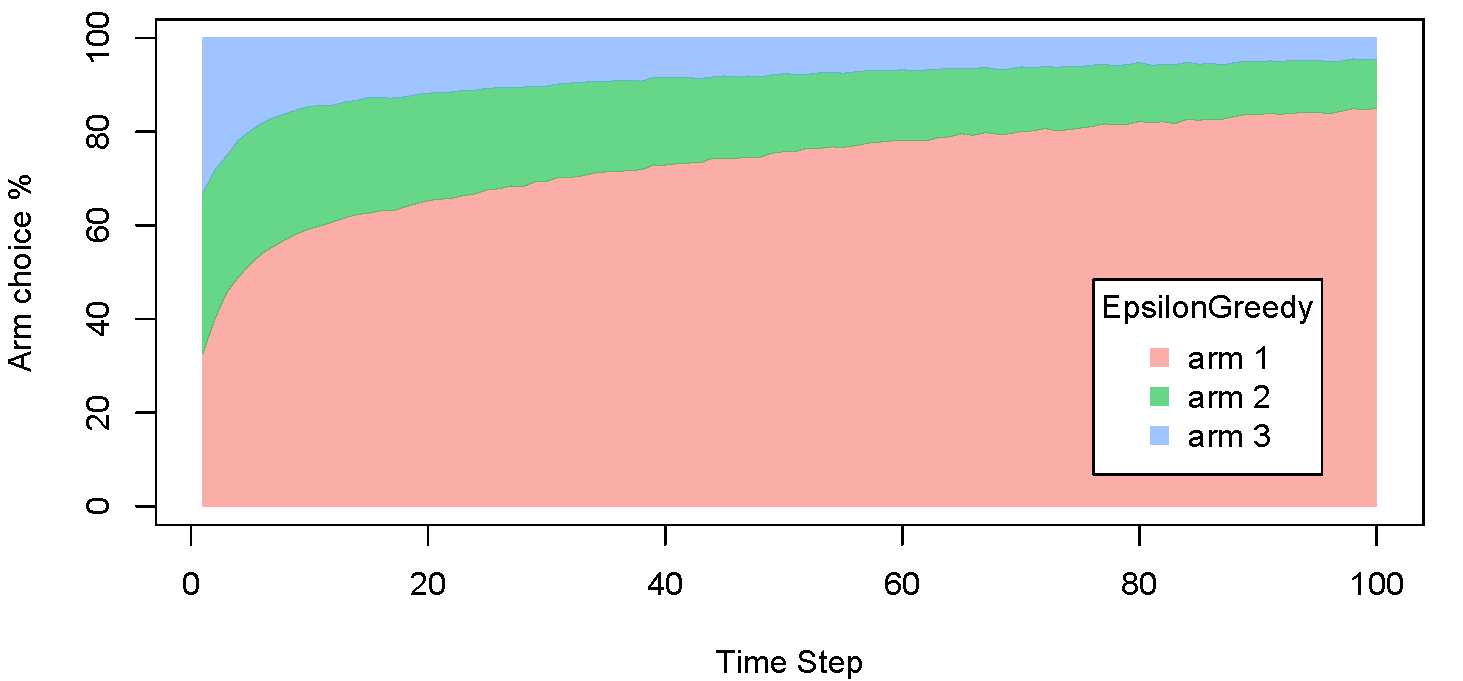
\includegraphics[width=.99\textwidth]{fig/section_2_3}
\label{fig:section_2_3}
\end{figure}


\section{Basic Usage} \label{basicusage}

The current section offers an overview of \pkg{contextual}'s predefined bandits and policies and further demonstrates how to run them.

\subsection{Implemented Policies and Bandits} \label{implbp}

Though contextual is at its most useful when developing and evaluating custom bandit and policy classes, as demonstrated in the previous section, it is also possible to run basic simulations with just its built-in bandits and policies. See Table \ref{table:overview_policies} for an overview of all available policies and Table \ref{table:overview_bandits} for an overview of all currently implemented bandits---where possible with references to their original papers.

\begin{table}[H]
\begin{tabularx}{\textwidth}{@{}lllllX@{}}
\toprule
\parnoteclear % tabularx will otherwise add each note thrice
& \textbf{$\epsilon$-Greedy} & \textbf{UCB} & \textbf{Thomspon Sampling} & \textbf{Other} & \textbf{Special} \\ \midrule
MAB & \begin{tabular}[c]{@{}l@{}}$\epsilon$-Greedy\parnote{\cite{Sutton1998e}}\\ $\epsilon$-First \end{tabular} & \begin{tabular}[c]{@{}l@{}}UCB1\parnote{\cite{Auer2002}} \\ UCB-tuned\parnote{\cite{Auer2002}} \end{tabular} & \begin{tabular}[c]{@{}l@{}}Thompson Sampling\parnote{\cite{Agrawal2011}} \\ BootstrapTS\parnote{\cite{Eckles2014}} \end{tabular} & \begin{tabular}[c]{@{}l@{}}Softmax\parnote{\cite{Vermorel2005}}\\ Gittins\parnote{\cite{Brezzi2002}}\end{tabular} & \multirow{2}{*}{\begin{tabular}[c]{@{}l@{}}Random\\ Oracle\\ LiF\parnote{\cite{Kaptein2016a}}\end{tabular}} \\ \cmidrule(r){1-5}
CMAB & Epoch-Greedy\parnote{\cite{Langford2008}} & \begin{tabular}[c]{@{}l@{}}LinUCB\parnote{\cite{Li2010}} \\ COFIBA\parnote{\cite{Li2016}}\end{tabular} & \begin{tabular}[c]{@{}l@{}}LinTS\parnote{\cite{Agrawal2012a}} \\ LogitBTS\parnote{\cite{Eckles2014}} \end{tabular} & & \\ \bottomrule
\end{tabularx}

\caption{An overview of \pkg{contextual}'s predefined policy classes.}
\label{table:overview_policies}
\end{table}

\begin{table}[H]
\begin{tabularx}{\textwidth}{@{}lllll@{}}
\toprule
\textbf{MAB} & \textbf{CMAB} & \textbf{Offline} & \textbf{Continuous} \\ \midrule
\begin{tabular}[t]{@{}l@{}}BasicBernoulliBandit\\ BasicGaussianBandit\end{tabular}  & \begin{tabular}[t]{@{}l@{}}ContextualBernoulli\\ ContextualLogit\\ ContextualHybrid\\ ContextualLinear\\ContextualWheel\parnote{\cite{Riquelme2018}}\end{tabular} & \begin{tabular}[t]{@{}l@{}}OfflinePolicyEvaluator\parnote{\cite{Li2011}}\\ DoublyRobust\parnote{\cite{Dudik2011}}\end{tabular} & ContinuumBandit \\ \bottomrule
\end{tabularx}
\caption{An overview of \pkg{contextual}'s predefined bandit classes.}
\label{table:overview_bandits}
\end{table}

\parnotes

\subsection{Running basic simulations} \label{basicsc}

In the current subsection we demonstrate how run simulations with \pkg{contextual}'s predefined bandit and policy classes on the basis of a familiar bandit scenario.

\subsubsection{The scenario} \label{scen}

As online advertising is one of the areas where bandit policies have found widespread application, we will use it as a backdrop to our basic bandit tutorial. Generally, the goal in online advertising is to determine which out of several ads to serve a visitor to a particular web page. Translated to a bandit setting, in online advertising:

\begin{itemize}
         \item The context is usually determined by visitor and web page characteristics.
         \item Arms are represented by the pool of available ads.
         \item An action is the displayed add as chosen by a policy.
         \item The reward is a visitor's click (a reward of 1) or non-click (a reward of 0) on an ad.
\end{itemize}

In the case of the simulations in the current section, we limit the number of advertisements in the pool to 3, and set ourselves the goal of finding the policy that offers the highest overall click-through rate within 400 impressions---with the higher level goal of choosing the best policy to implement on a live website.

\subsubsection{Comparing context-free policies} \label{ncp}

Before we are able to evaluate any policies, we first have to model the three ads---with each a different probability of generating a click---as the arms of a bandit. We choose to model the ads with the weight-based \code{SyntheticBandit} as this enabled us to easily set uniformly distributed weights determining the probability of the rewards for each arm. As can be observed in the source code below, for the current simulation, we set the weights of the arms to respectively $p = 0.8$, $p = 0.4$ and $p = 0.2$.

We also choose two context-free policies to evaluate and compare:

\begin{itemize}
         \item \code{EpsilonFirstPolicy}: explores all three ads at uniformly at random for a preset period and from thereon exploits the ad with the best click-through rate \footnote{A type of policy also known as an A/B test \cite{Kohavi2007}.}. For our current scenario, we set the exploration period to 50 impressions. A formal definition and an implementation of the algorithm can be found in section \ref{epsfirst}.

         \item \code{EpsilonGreedyPolicy}: explores one of the ads at uniformly at random $\epsilon$ of the time and exploits the ad with the best current click-through rate $1 - \epsilon$ of the time. For our current scenario, we set $\epsilon = 0.2$. For a formal definition and implementation see section \ref{epsgreedy}.
\end{itemize}

Next, we assign the one \code{bandit} instance and two \code{policy} instances to two \code{agents}, ensuring that both policies are run on the same set of generated data. Finally, we assign a \code{list} holding both \code{agents} to a \code{Simulator} instance, set the \code{simulator}'s horizon to 400 and the number of repeats to 1000, run the simulation, and \code{plot()} its results:

\begin{Code}
# Load and attach the contextual package.
library(contextual)
# Define for how long the simulation will run.
horizon             <- 400
# Define how many times to repeat the simulation.
simulations         <- 1000
# Define the probability that each ad will be clicked.
click_probabilities <- c(0.8, 0.4, 0.2)
# Initialize a SyntheticBandit, which takes probabilites per arm for an argument.
bandit              <- SyntheticBandit$new(weights = click_probabilities)
# Initialize an EpsilonGreedyPolicy with a 20% exploiration rate.
eg_policy           <- EpsilonGreedyPolicy$new(epsilon = 0.2)
# Initialize an EpsilonFirstPolicy with a 50 step exploration period.
ef_policy           <- EpsilonFirstPolicy$new(first = 50)
# Initialize two Agents, binding each policy to a bandit.
ef_agent            <- Agent$new(ef_policy, bandit)
eg_agent            <- Agent$new(eg_policy, bandit)
# Assign both agents to a list.
agents              <- list(ef_agent, eg_agent)
# Initialize a Simulator with the agent list, horizon, and number of simulations.
simulator           <- Simulator$new(agents, horizon, simulations)
# Now run the simulator.
history             <- simulator$run()
# And plot the cumulative reward rate (equals Click Through Rate)
plot(history, type = "cumulative", regret = FALSE, rate = TRUE)
\end{Code}
\begin{figure}[H]
\centering
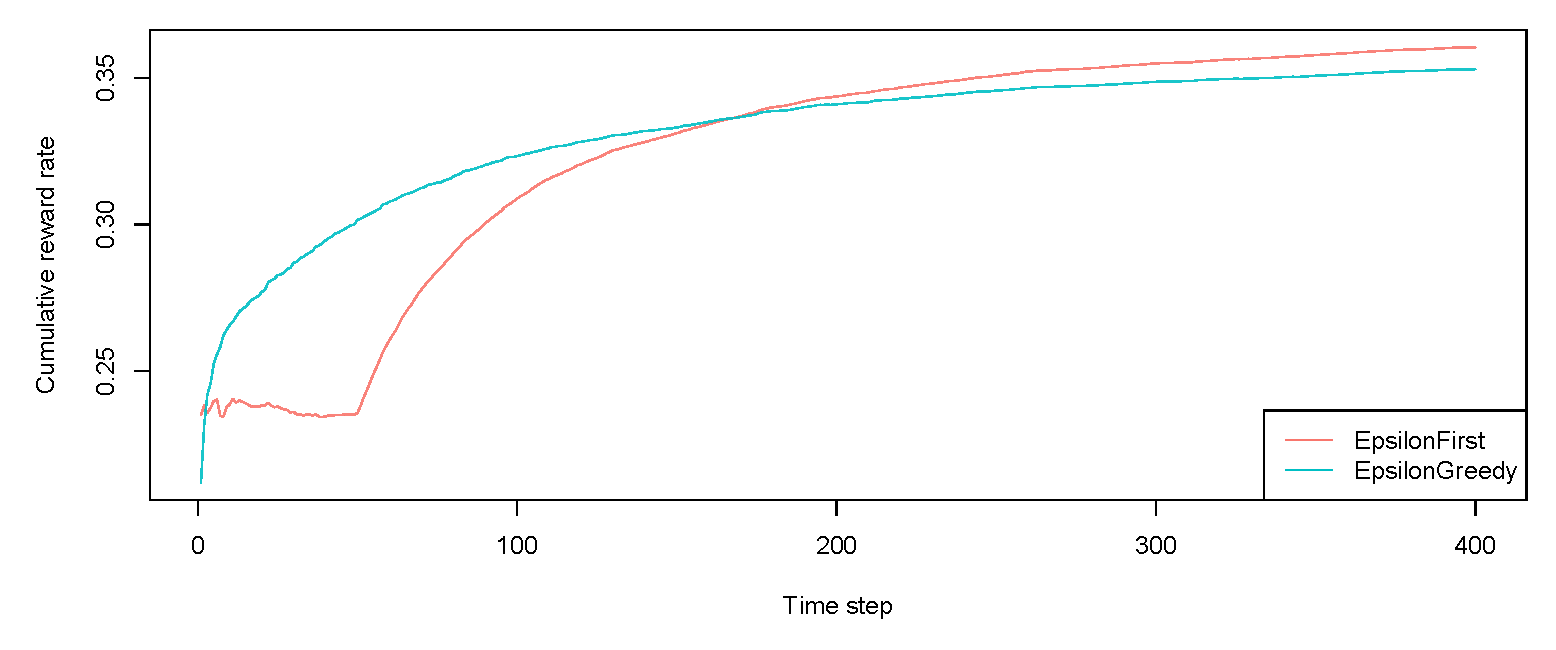
\includegraphics[width=.99\textwidth]{fig/simple_one}
\label{fig:simple_one}
\caption{Cumulative reward rate (equals click-through rate) of a context-free bandit scenario comparing $\epsilon$-first and $\epsilon$-greedy policies.}
\end{figure}

As can be observed in Figure \ref{fig:simple_one}, within our horizon of $T = 400$, \code{EpsilonFirstPolicy} has accumulated more rewards than \code{EpsilonGreedytPolicy}. It is easy to see why: The winning arm is consistently the best - by a margin.  So \code{EpsilonFirstPolicy} has no difficulty in finding the optimal arm within its exploration period of 50 impressions. Up to that point, \code{EpsilonGreedyPolicy} had the advantage of a headstart---from the moment it established which arm was best, it was able to exploit it for $1- \epsilon$ or 80 percent of the time. However, in contrast to \code{EpsilonFirstPolicy}, it is not able to exploit it consistently from 50 impressions on---the \code{EpsilonGreedyPolicy} is obliged to keep exploring lesser arms for 20 percent of the time.

\subsubsection{Adding context}

If that is all we know of our visitors, we expect the results to be stationary over time, and these are the only policies available, the choice is clear: we will use \code{EpsilonFirstPolicy} on our live website\footnote{Also: if our bandit represents our visitors' click behavior realistically, if our policies' parameters are optimal, etcetera.}. However, if we have contextual information on our visitors---for instance, their age---we might be able to do better. Let us suggest, for instance, that we expect that some of our ads are more effective for older visitors, and other ads more effective for younger visitors.

To incorporate this expectation in our simulation, we need to change the way our bandit generates its rewards. Fortunately, in the case of our \code{SyntheticBandit}, the introduction of two contextual features only requires the addition of a single row to its weight matrix---as \code{SyntheticBandit} parses each of the $d$ rows of its weight matrix as a binary feature generated with a probability of $p_{d,t} = 1/d$.

As can be seen in the source code below, in choosing our weights, we have taken care to keep the average rewards per arm over the two features equal to the rewards per arm in the previous simulation. So we do not expect a substantial difference with the previous simulation's outcome for context-free policies \code{EpsilonFirstPolicy} and \code{EpsilonGreedyPolicy}.

We therefore also include the contextual \code{LinUCBDisjointPolicy} \citep{Li2010}, which, in assuming its reward function is a linear function of the context, is able to incorporate our new contextual information into its decision-making process. See \ref{linucbc} for a detailed description and implementation details of this policy. Now let us rerun the simulation:


\begin{Code}
#                                    +-----+----+-----------> ads: k = 3
#                                    |     |    |
click_probabilities <- matrix(  c(  0.2,  0.3, 0.1,     # --> d1: old   (p=.5)
                                    0.6,  0.1, 0.1   ), # --> d2: young (p=.5)
                                                        #     features: d = 2

                                  nrow = 2, ncol = 3, byrow = TRUE)

# Initialize a SyntheticBandit with contextual weights
context_bandit      <- SyntheticBandit$new(weights = click_probabilities)
# Initialize LinUCBDisjointPolicy
lu_policy           <- LinUCBDisjointPolicy$new(0.6)
# Initialize three Agents, binding each policy to a bandit.
ef_agent            <- Agent$new(ef_policy, context_bandit)
eg_agent            <- Agent$new(eg_policy, context_bandit)
lu_agent            <- Agent$new(lu_policy, context_bandit)
# Assign all agents to a list.
agents              <- list(ef_agent, eg_agent, lu_agent)
# Initialize a Simulator with the agent list, horizon, and number of simulations.
simulator           <- Simulator$new(agents, horizon, simulations)
# Now run the simulator.
history             <- simulator$run()
# And plot the cumulative reward rate again.
plot(history, type = "cumulative", regret = FALSE, rate = TRUE)
\end{Code}
\begin{figure}[H]
\centering
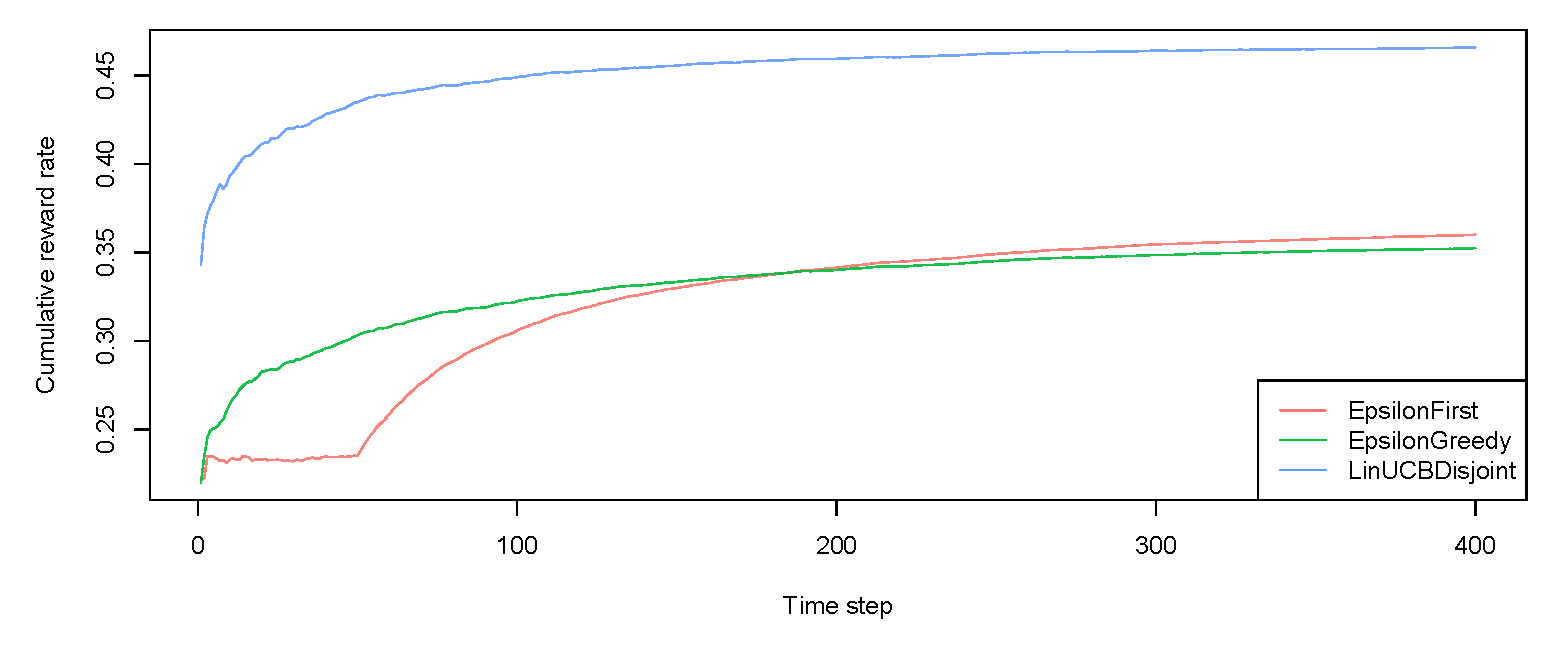
\includegraphics[width=.99\textwidth]{fig/simple_two}
\label{fig:simple_two}
\caption{Cumulative reward rate (equals click-through rate) of a contextual bandit scenario comparing LinUCB, $\epsilon$-first and $\epsilon$-greedy policies.}
\end{figure}

As can be observed in Figure \ref{fig:simple_two}, both context-free bandit's results do indeed about as well as before. On the other hand, \code{LinUCBDisjointPolicy} does very well, as this contextual policy is able to map its rewards to the observed contextual features. All in all, this time around, you would probably choose the \code{LinUCBDisjointPolicy} for your website---with the added advantage of being able to incorporate other contextual features to optimize results further.

Of course, neither simulation in the current section is very realistic. One way to do better would be to write a Bandit subclass with a more complex generative model. How to create such a bandit subclass is delineated in section 5. Another option would, for example, be to evaluate policies on an offline dataset---more on that in section 6.

\section{Class structure} \label{classstructure}

Since it is \pkg{contextual}'s explicit goal to offer researchers and developers an easily extensible framework to develop, evaluate and compare their own \code{Policy} and \code{Bandit} implementations, the current section offers additional background information on \pkg{contextual}'s class structure---both on the R6 class system \cite{R6} and on each of the six previously introduced core \pkg{contextual} classes.

\subsection{Choice for the R6 Class System} \label{classsystem}

Though widely used as a procedural language, \proglang{R} offers several Object Oriented (OO) systems, which can significantly help in structuring the development of more complex packages. Out of the OO systems available (S3, S4, R5 and R6), we settled on R6, as it offered several advantages compared to the other options. Firstly, it implements a mature object-oriented \footnote{In object-oriented programming, the developer compartmentalizes data into objects, whose behavior and contents are described through the declaration of classes. Its benefits include reusability, refactoring, extensibility, ease of maintenance and efficiency. See, for instance, \cite{Wirfs-Brock1990} for a general introduction to the princples of Object Oriented software design, and \cite{wickham2014advanced} for more information of the use of OOP in \proglang{R}.} design when compared to S3. Secondly, its classes can be accessed and modified by reference---which offers the added advantage that R6 classes are instantly recognizable for developers with a background in programming languages such as \proglang{Java} or \proglang{C++}. Finally, when compared to the older R5 reference class system, R6 classes are lighter-weight and (as they do not make use of S4 classes) do not require the methods package---which makes \pkg{contextual} substantially less resource-hungry than it would otherwise have been.

\subsection{Main Classes} \label{mainclasses}

In this section, we go over each of \pkg{contextual}'s six main classes in some more detail---with an emphasis on the \code{Bandit} and \code{Policy} classes. To clarify \pkg{contextual}'s class structure, we also include two UML diagrams (UML, or "unified modeling language" presents a standardized way to visualize the overall class structure and general design of a software application or framework \citep{Rumbaugh2004}). The UML class diagram shown in Figure \ref{fig:contextual_class} on page \pageref{fig:contextual_class} visualizes \pkg{contextual}'s static object model, showing how its classes inherit from, and interface with, each other. The UML sequence diagram in figure Figure \ref{fig:contextual_sequence} on page \pageref{fig:contextual_sequence}, on the other hand, illustrates how \pkg{contextual}'s classes interact dynamically over time.

\subsubsection{Bandit}

In \pkg{contextual}, any bandit implementation is expected to subclass and extend the \code{Bandit} superclass. It is then up to these subclasses themselves to provide an implementation for each of its abstract methods. In practice, this entials that \code{Bandit} subclasses are, firstly, responsible for setting the instance variable \code{self\$k} to the number of arms, and instance variable \code{self\$d} to the number of context features. Next, any \code{Bandit} siblings are expected to implement at least \code{get_context()} and \code{do_action()}:

\begin{Code}
#' @export
Bandit <- R6::R6Class(
  portable = TRUE,
  class    = FALSE,
  public   = list(
    k           = NULL,     # Number of arms (integer)
    d           = NULL,     # Dimension of context feature vectors (integer)
    ...
    precaching  = FALSE,    # Pregenerate context & reward matrices? (boolean)
    class_name  = "Bandit", # Bandit name - required (character)
    initialize  = function() {
      # Initialize Bandit. Set self$d and self$k here.
    },
    ...
    get_context = function(t) {
      stop("Bandit subclass needs to implement bandit$get_context()", call. = FALSE)
      # Return a list with self$k, self$d and, where applicable, a context matrix X.
      list(X = context, k = arms, d = features)
    },
    get_reward = function(t, context, action) {
      stop("Bandit subclass needs to implement bandit$get_reward()", call. = FALSE)
      # Return a list with the reward and, if known, the reward of the best arm.
      list(reward = reward_for_choice_made, optimal = optimal_reward_value)
    },
    ...
  )
)
\end{Code}


The main \code{Bandit} functions can be futher detailed as follows:

\begin{itemize}
  \item{\code{new()}}{ Generates and initializes a new \code{Bandit} object. }
  \item{\code{pre_calculate()}}{
     Called right after \code{Simulator} sets its seed,
     but before it starts iterating over all time steps \code{t} in T. If you need to initialize random values in a \code{Policy},
     this is the place to do so.
  }
  \item{\code{get_context(t)}}{
     Returns a named list \code{list(k = n_arms, d = n_features, X = context)}
     with the current \code{d x k} dimensional \code{context} feature matrix \code{X} together with the number of arms \code{k}.
 }
  \item{\code{get_reward(t, context, action)}}{
     Returns the named list \code{list(reward = reward_for_choice_made,
     optimal = optimal_reward_value)} containing the \code{reward}
     for the \code{action} previously returned by \code{policy} and,
     optionally, the \code{optimal} reward
     at the current time \code{t}.
 }
  \item{\code{generate_bandit_data()}}{
     A helper function that is called before \code{Simulator} starts iterating over all time steps \code{t} in T.
     This function is called when \code{bandit$precaching} has been set to \code{TRUE}.
     Pregenerate \code{contexts} and \code{rewards} here.
  }
\end{itemize}

As already previously indicated in Table \ref{table:overview_bandits} from Section 3.1 \code{Bandit}, \pkg{contextual} already contains several predefined Bandits. For each of these Bandits, the package offers at least one example script, to be found in the package’s demo directory:

\begin{itemize}
         \item \code{BasicBandit}: this basic (context-free) k-armed bandit synthetically generates rewards based on a weight vector. It returns a unit vector for context matrix X.
                  \item \code{SyntheticBandit}: an example of a more complex and versatile synthetic bandit. It pregenerates both a randomized context matrix and reward vectors
         \item \code{ContextualBandit}: a contextual bandit that synthetically generates contextual rewards based on randomly set weights. It can simulate mixed user (cross-arm) and article (arm) feature vectors, generated from parameters k, d and num\_users.
         \item \code{ContinuumBandit}: a basic example of a continuum bandit.
         \item \code{LiBandit}: a basic example of a bandit that makes use of offline data - here, an implementation of Li's [reference].
\end{itemize}

Each of these bandits can be deployed to run policies without further ado. They can, however, also be used as either examples or templates for your own custom \code{Bandit} implementation(s), or as superclasses for sub-subclass implementations.

\subsubsection{Policy}

\code{Policy} is the second often subclassed contexual superclass. Just like the \code{Bandit} superclass, \code{Policy} is an abstract class that declares methods without itself offering an implementation. Any \code{Policy} subclass is therefore expected to implement \code{get_action()} and \code{set_reward()}. Also, any parameters that keep track or summarize \code{context}, \code{action} and \code{reward} values are required to be saved to \code{Policy}'s \textit{named list} \code{theta}.

\begin{Code}
#' @export
Policy <- R6::R6Class(
  portable = FALSE,
  class = FALSE,
  public = list(
    action        = NULL,      # action results (list)
    theta         = NULL,      # policy parameters theta (list)
    theta_to_arms = NULL,      # theta to arms "helper" (list)
    class_name    = "Policy",  # policy name - required (character)
    initialize = function() {
      self$theta  <- list()    # initializes theta list
      self$action <- list()    # initializes action list
    },
    get_action = function(t, context) {
      # Selects an arm based on self$theta and context, returns it in action$choice
      stop("Policy$get_action() has not been implemented.", call. = FALSE)
    },
    set_reward = function(t, context, action, reward) {
      # Updates parameters in theta based on reward awarded by bandit
      stop("Policy$set_reward() has not been implemented.", call. = FALSE)
    },
    set_parameters = function(context_params) {
      # Policy parameter (not theta!) initialisation happens here
      stop("Policy$set_parameters() has not been implemented.", call. = FALSE)
    },
    initialize_theta = function(k) {
      # Called during contextual's initialisation.
      # Copies theta_to_arms k times, makes the copies available through theta.
      ...
    }
  )
)
\end{Code}

\code{Policy}'s main functions can be futher detailed as follows:

\begin{itemize}

\item{\code{set_parameters()}}{
 This helper function, called during a \code{Policy}'s initialisation, assigns the values
 it finds in list \code{self$theta_to_arms} to each of the \code{Policy}'s k arms.
 The parameters defined here can then be accessed by arm index in the following way:
 \code{theta[[index_of_arm]]$parameter_name}. The source code in section \ref{epsfirst}
 illustrates the mechanism further.
}

\item{\code{get_action(t, context)}}{
 Calculates which arm to play based on the current values in named list \code{theta}
 and the current \code{context}. Returns a named list
 \code{list(choice = arm_chosen_by_policy)} that holds the index of the arm
 to play.
}

\item{\code{set_reward(t, context, action, reward)}}{
 Returns the named list
 \code{list(reward = reward_for_choice_made, optimal = optimal_reward_value)} containing the \code{reward}
 for the \code{action} previously returned by \code{policy} and, optionally, the \code{optimal} reward
 at the current time \code{t}.
 }
\end{itemize}

\subsubsection{Agent}

To ease the encapsulation of parallel \code{Bandit} and \code{Policy} simulations, \code{Agent} is responsibe for the flow of information between and the running of one \code{Bandit} and \code{Policy} pair, for example:

\begin{Code}
policy             <- EpsilonGreedyPolicy$new(epsilon = 0.1, name = "EG")
bandit             <- SyntheticBandit$new(weights = c(0.9, 0.1, 0.1))
agent              <- Agent$new(policy,bandit)
\end{Code}

It does this by keeping track of \code{t}  through its private named list variable \code{state} and by making sure that, at each time step \code{t}, all four main \code{Bandit} and \code{Policy} CMAB methods are called in correct order, one after the other:

\begin{Code}
Agent <- R6::R6Class(
  public = list(
    #...
    do_step = function() {
      t <- t + 1
      context = bandit$get_context(t)
      action  = policy$get_action (t, context)
      reward  = bandit$get_reward (t, context, action)
      theta   = policy$set_reward (t, context, action, reward)
      list(context = context, action = action, reward = reward,theta = theta)
    }
    #...
  )
)
\end{Code}

Its main function is \code{do_step()}, generally called by a \code{Simulator} object (or, more specifically, by the \code{Simulator}-started parallel worker that is repsonsible for this particular \code{Agent}):

\begin{itemize}
   \item{\code{do_step()}}{
      Completes one time step \code{t} by consecutively calling
      \code{bandit$get_context()}, \code{policy$get_action()}, \code{bandit$get_reward()} and \code{policy$set_reward()}.
    }
\end{itemize}

\subsubsection{Simulator}

A \code{Policy} instance is the entry point of any \pkg{contextual} simulation. It encapsulates one or more \code{Agents}, clones them if necessary, runs the \code{Agents} (in parallel, by default), and saves the log of all of the \code{Agents} interactions to a \code{History} object:

\begin{Code}
history <- Simulator$new(agents = agent, horizon = 10, simulations = 10)$run()
\end{Code}

By default, for performance reasons, a \code{Simulator} does not save \code{context} matrices and the (potentially deeply nested) \code{theta} list to its \code{History log}---though this can be changed  by setting either \code{save_context} and \code{save_theta} arguments set to \code{TRUE}.

To specify how to run a simulation and which data is to be saved to a \code{Simulator} instance's \code{History} log, a \code{Policy} object can be configured through the following parameters:

\begin{itemize}
   \item{\code{agents}}{
     An \code{Agent} instance, or a \code{list} of \code{Agent} instances to be run by the instantiated \code{Simulator}.
   }
   \item{\code{horizon}}{
     The T time steps to run the instantiated \code{Simulator}.
   }
   \item{\code{simulations}}{
     How many times to repeat each agent's simulation with a new seed on each repeat (itself deterministically derived from set\_seed).
   }
   \item{\code{save_context}}{
     Save context matrices \code{X} to the \code{History} log during a simulation?
   }
   \item{\code{save_theta}}{
     Save the parameter list \code{theta} to the \code{History} log during a simulation?
   }
   \item{\code{do_parallel}}{
      Run \code{Simulator} processes in parallel?
   }
   \item{\code{worker_max}}{
      Specifies how many parallel workers are to be used, when \code{do_parallel} is \code{TRUE}. If unspecified, the amount of workers defaults to \code{max(workers_available)-1}.
   }
   \item{\code{continuous_counter}}{
      Of use to offline Bandits.
      If \code{continuous_counter} is set to \code{TRUE}, the current \code{Simulator}
      iterates over all rows in a dataset for each repeated simulation.
      If \code{FALSE}, it splits the data into \code{simulations} parts,
      and a different subset of the data for each repeat of an agent's simulation.
   }
   \item{\code{set_seed}}{
      Sets the seed of \proglang{R}'s random number generator for the current \code{Simulator}.
   }
   \item{\code{write_progress_file}}{
       If \code{TRUE}, \code{Simulator} writes \code{progress.log} and \code{doparallel.log}
       files to the current working directory, allowing you to keep track of \code{workers}, iterations,
       and potential errors when running a \code{Simulator} in parallel.
   }
   \item{\code{include_packages}}{
       List of packages that (one of) the policies depend on. If a \code{Policy} requires an
       \proglang{R} package to be loaded, this option can be used to load that package on each of the workers.
       Ignored if \code{do_parallel} is \code{FALSE}.
   }
   \item{\code{reindex}}{
      If \code{TRUE}, removes empty rows from the \code{History} log,
      re-indexes the \code{t} column, and truncates the resulting data to the shortest simulation
      grouped by agent and simulation.
   }
\end{itemize}

\subsubsection{History}

A \code{Simulator} aggregates the data acquired during a simulation in a \code{History} object's private \code{data.table} log. It also calculates per agent average cumulative reward, and, when the optimal outcome per \code{t} is known, per agent average cumulative regret. It is furthermore possible to \code{plot()} a \code{History object}, \code{summarize()} it, or obtain, for example, a \code{data.frame()} or a \code{data.table()} from any \code{History} instance:

\begin{Code}
history             <- Simulator$new(agent)$run()
dt                  <- history$get_data_table()
df                  <- history$get_data_frame()
cumulative_regret   <- history$cumulative(regret = TRUE)
\end{Code}

Some other \code{History} functions:

\begin{itemize}
 \item{\code{set(index,
                  t,
                  action,
                  reward,
                  policy_name,
                  simulation_index,
                  context_value = NA,
                  theta_value = NA)}}{
    Stores one row of simulation data. Generally not called directly,
    but rather through a \code{Simulator} instance.
 }
 \item{\code{save(filename = NA)}}{
    Writes \code{History} to a file with name \code{filename}.
 }
 \item{\code{load(filename, interval = 0)}}{
    Reads a \code{History} log file with name \code{filename}.
    If \code{interval} is larger than 0, every other \code{interval} row of data is read instead of the
    full data file.
 }
 \item{\code{reindex(truncate = TRUE)}}{
    Removes empty rows from the \code{History} log, reindexes the \code{t} column, and,
    when \code{truncate} is \code{TRUE}, truncates the resulting data to the number of rows of the shortest
    simulation.
 }
\end{itemize}

\subsubsection{Plot}

The \code{Plot} class takes an \code{History} object and offers several ways to plot it, each optimized to be able to plot gigabytes worth of data, quickly:

\begin{itemize}
         \item \code{average}: plots the average reward or regret over all simulations per Agent (that is, each \code{Bandit} and Policy combo) over time.
         \item \code{cumulative}: plots the average reward or regret over all simulations per Agent over time.
         \item \code{arms}: plots ratio of arms chosen on average at each time step, in percentages, totaling 100%.

\end{itemize}

\code{Plot} objects can be instantiated directly, or, more commonly, by calling the \code{plot()} function. In either case, make sure to specify a \code{History} instance and one of the plot types specified above:

\begin{Code}
# plot a history object through default generic plot() function
plot(history, type = "arms")

# or call the Plot() directly
p1 <- Plot$new()$cumulative(history)
p2 <- Plot$new()$average(history)
\end{Code}

Multiple agents can be combined within one \code{Plot}, and multiple plots can themselves again be combined into one graph by turning off the default \code{par} formatting of the \code{Plot} class and redefining \code{par} through, for example \code{par(mfrow, mar)}. Some example plots that illustrate many of \code{Plot()}'s features:

\begin{Code}
bandit             <- SyntheticBandit$new(weights = c(0.9, 0.1, 0.1))
agents             <- list(Agent$new(RandomPolicy$new(), bandit),
                           Agent$new(OraclePolicy$new(), bandit),
                           Agent$new(ThompsonSamplingPolicy$new(1.0, 1.0), bandit),
                           Agent$new(Exp3Policy$new(0.1), bandit),
                           Agent$new(GittinsBrezziLaiPolicy$new(), bandit),
                           Agent$new(UCB1Policy$new(), bandit))
history            <- Simulator$new(agents, horizon = 100, simulations = 1000)$run()
par(mfrow = c(3, 2), mar = c(5, 5, 1, 1))
plot(history, type = "cumulative", use_colors = FALSE, no_par = TRUE)

plot(history, type = "cumulative", regret = FALSE, legend = FALSE,
     limit_agents = c("UCB1"), traces = TRUE, no_par = TRUE)

plot(history, type = "cumulative", regret = FALSE, rate = TRUE, ci = "sd",
     limit_agents = c("Exp3", "ThompsonSampling"),
     legend_position = "bottomright", no_par = TRUE)

plot(history, type = "cumulative", rate = TRUE, plot_only_ci = TRUE,
     ci = "var", smooth = TRUE, limit_agents = c("UCB1", "GittinsBrezziLai"),
     legend_position = "topright", no_par = TRUE)

plot(history, type = "average", ci = "ci", regret = FALSE, interval = 10,
     smooth = TRUE, legend_position = "bottomright", no_par = TRUE)

plot(history, limit_agents = c("ThompsonSampling"), type = "arms",
     interval = 20, no_par = TRUE)
par(mfrow = c(1, 1))
\end{Code}
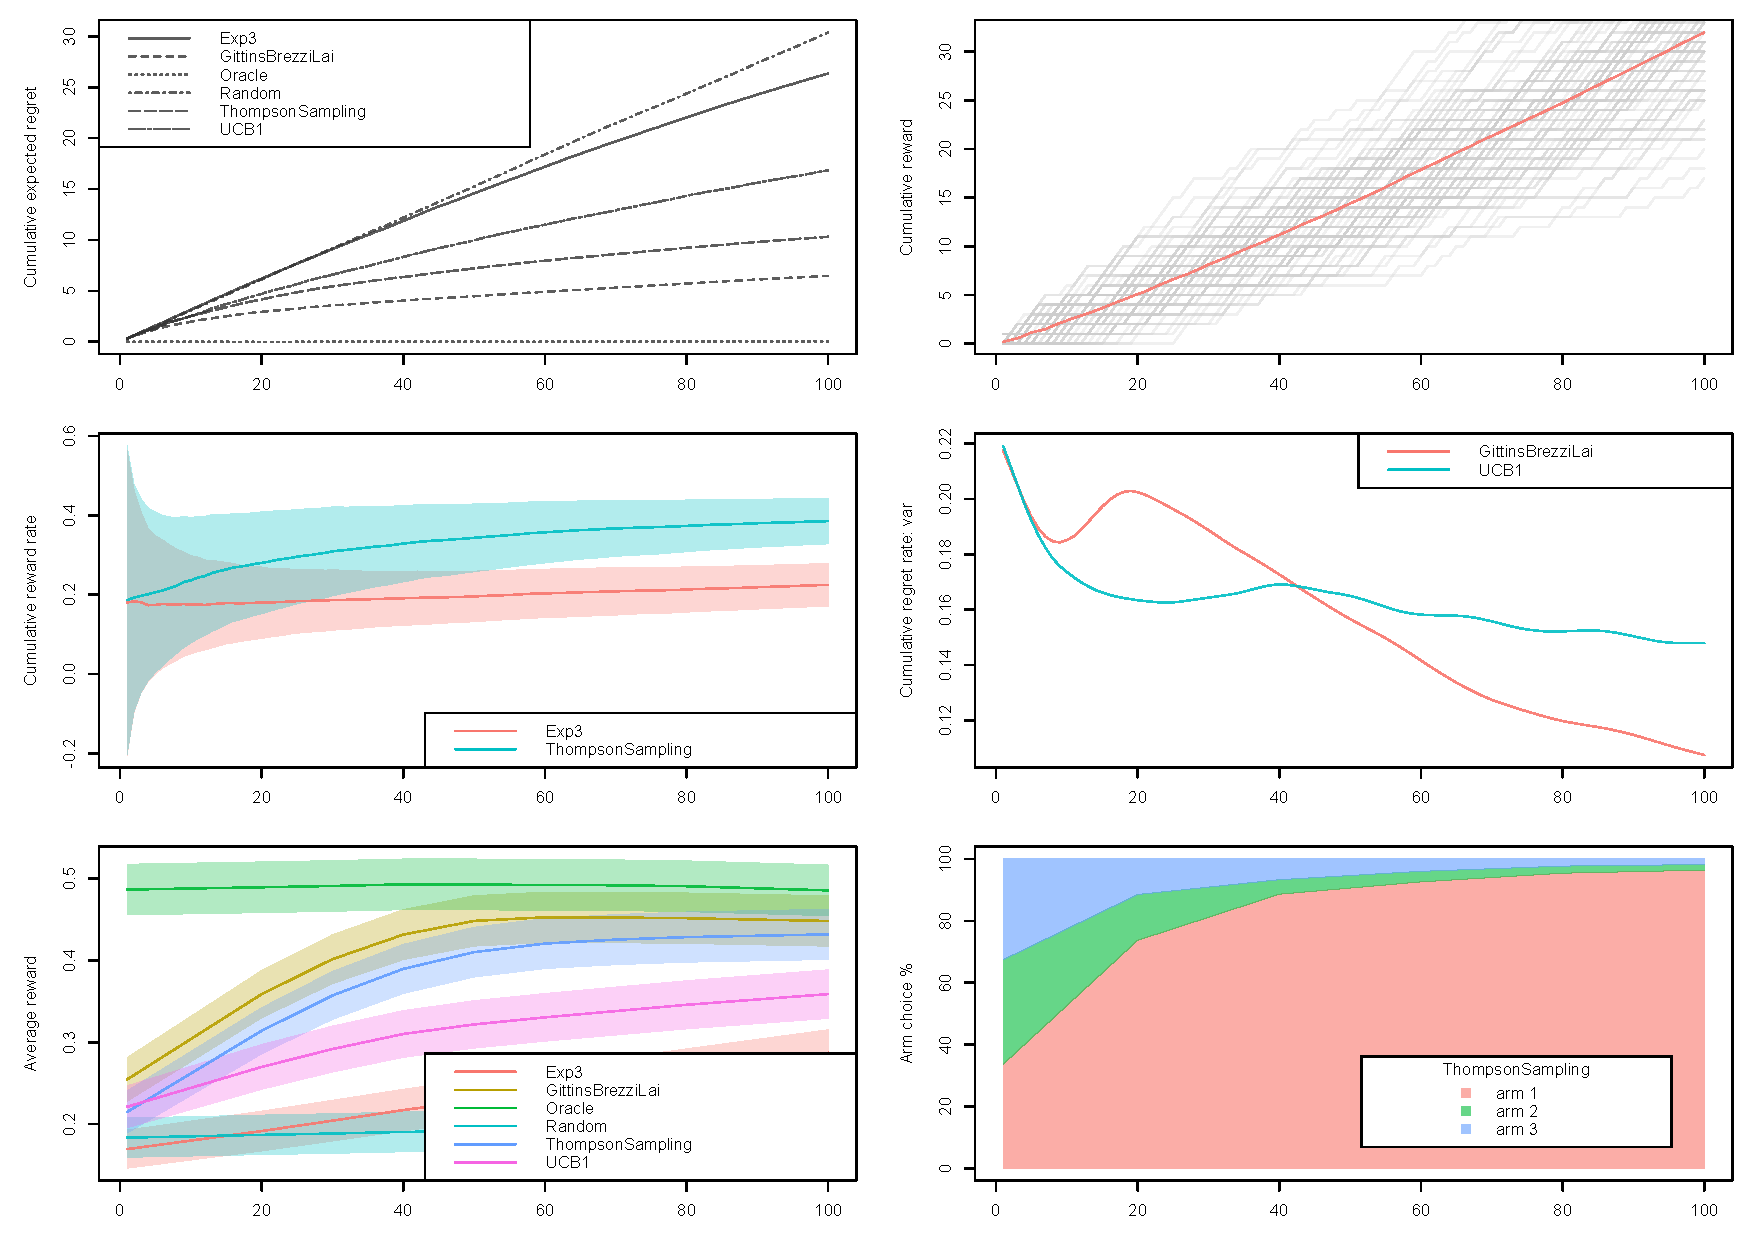
\includegraphics[width=\textwidth]{fig/plot_examples}

\section{Implementing and extending Policy and Bandit subclasses} \label{extending}

Though section 3 provides a first introduction to all of \pkg{contextual}'s main classes, in practice, researchers will mostly focus on subclassing \code{Policies} and \code{Bandits}. The current section therefore first demonstrates how to implement some well-known bandit algorithms, and, secondly, how to create \code{Policy} and \code{Bandit} sub-subclasses.

\subsection{BasicBandit: a Minimal Bernoulli Bandit} \label{basicbandit}

Where not otherwise noted, all \code{Bandit} implementations in the current paper refer to (or will be configured as) multi-armed \code{Bandits} with Bernoulli rewards. For Bernoulli \code{Bandits}, the reward received is either a zero or a one: on each $t$ they offer either a reward of $1$ with probability $p$ or a reward of $0$ with probability $1 - p$. In other words, a Bernoulli bandit has a finite set of arms a \(  \in \left\{ 1, \dots, k \right\} \) where the rewards for each arm $a$ is distributed Bernoulli with parameter $p_a$, the expected reward of the arm.

One example of a very simple context-free Bernoulli bandit is \pkg{contextual}'s minimal \code{Bandit} implementation, \code{BasicBandit}:

\begin{Code}
BasicBandit <- R6::R6Class(
  inherit = Bandit,
  public = list(
    initialize   = function(weights = NULL) {
      self$set_weights(weights)                         # arm weight vector
      private$X <- array(1, dim = c(self$d, self$k, 1)) # context matrix of ones
    },
    # ...
    get_weights = function() {
      private$W
    },
    set_weights = function(local_W) {
      private$W <- matrix(local_W, nrow = 1L)           # arm weight vector
      self$d    <- as.integer(dim(private$W)[1])        # context dimensions
      self$k    <- as.integer(dim(private$W)[2])        # arms
      private$W
    },
    get_context = function(t) {
      contextlist <- list(k = self$k, d = self$d, X = private$X)
      contextlist
    },
    get_reward = function(t, context, action) {
      private$R  <- as.double(matrix(runif(self$k) < get_weights(), self$k, self$d))
      rewardlist <- list(
        reward                   = private$R[action$choice],
        optimal_reward_value     = private$R[which.max(private$R)]
      )
      rewardlist
    }
    # ...
  )
)
\end{Code}

\code{BasicBandit} expects a \code{weight} vector of probabilities, where every element in \code{weight} represents the probability of \code{BasicBandit} returning a reward of $1$ for one of its \code{k} arms. Also, observe that, at every \code{t}, \code{BasicBandit} sets private \code{context} matrix \code{X} to an unchanging, neutral \code{d} features times \code{k} arms unit matrix, which alludes to the fact that \code{BasicBandit} does not generate any covaried contextual cues related to its arms.

\subsection{EpsilonFirstPolicy} \label{epsfirst}

An important feature of \pkg{contextual} is that it eases the conversion from formal and pseudocode policy descriptions to clean R6 classes. We will give several examples of such conversions in the current paper, starting with the implementation of the $\epsilon$-first algorithm. In this context-free algorithm, also known as AB(C) testing, a pure exploration phase is followed by a pure exploitation phase.

In that respect, the $\epsilon$-first algorithm is equivalent to a randomized controlled trial (RCT). An RCT, generally refered to as the gold standard clinical research paradigm, is a study design where subjects are allocated at random to receive one of several clinical interventions. On completion of an RCT, the most succesful intervention up till that point in time is suggested to be the superior "evidence-based" option from then on.

A more formal pseudocode description of this $\epsilon$-first policy:

\begin{algorithm}[H]
\caption{$\epsilon$-first}
\label{Alg:EpsilonFirst}
\begin{algorithmic}
\REQUIRE \(   \eta \in \mathbb{Z}^{+} \)  , number of time steps $t$ in the exploration phase
\STATE \( n_{a} \leftarrow 0 \) for all arms a \(  \in \left\{ 1, \dots, k \right\} \)  (count how many times an arm has been chosen)
\STATE \( \hat{\mu}_{a} \leftarrow 0 \) for all arms a  \(   \in \left\{ 1, \dots, k \right\} \)  (estimate of expected reward per arm)
% Run through time points:
\FOR{$t=1, \dots, T$}
	% Run through arms. Step 1, select which one to play
	\IF {\(t \leq \eta\)}
	       \STATE play a random arm out of all arms a \(   \in \left\{ 1, \dots, k \right\} \)
	\ELSE
	        \STATE play arm \(a_t = \argmax_a  \hat{\mu}_{t=\eta,a}  \) with ties broken arbitrarily
	\ENDIF
	\STATE observe real-valued payoff $r_t$
	% Update:
	\STATE \( n_{a_{t}} \leftarrow n_{a_{t-1}} + 1  \)
   \STATE \( \hat{\mu}_{t,a_{t}} \leftarrow   \cfrac{r_t - \hat{\mu}_{t-1,a_{t}} }{n_{a_{t}}}   \)
\ENDFOR
\end{algorithmic}
\end{algorithm}

And the above pseudocode converted to an \code{EpsilonFirstPolicy} class:

\begin{Code}
EpsilonFirstPolicy <- R6::R6Class(
  public = list(
    first = NULL,
    initialize = function(first = 100) {
      super$initialize(name)
      self$first <- first
    },
    set_parameters = function() {
      self$theta_to_arms <- list('n' = 0, 'mean' = 0)

      # Here, we define a list with 'n' and 'mean' theta parameters to each arm
      # through helper variable self$theta_to_arms. That is, when the number of
      # arms is 'k', the above would equal:

      # self$theta <- list(n = rep(list(0,k)), 'mean' = rep(list(0,k)))

      # ... which would also work just fine, but is much less concise.

      # When assigning both to self$theta directly and via self$theta_to_arms,
      # do make sure to do it in that order.

    },
    get_action = function(context, t) {
      if (sum_of(theta$n) < first) {
        action$choice          <- sample.int(context$k, 1, replace = TRUE)
        action$propensity   <- (1/context$k)
      } else {
        action$choice          <- max_in(theta$mean, equal_is_random = FALSE)
        action$propensity   <- 1
      }
      action
    },
    set_reward = function(context, action, reward, t) {
      arm      <- action$choice
      reward   <- reward$reward

      inc(theta$n[[arm]]) <- 1
      if (sum_of(theta$n) < first - 1)
        inc(theta$mean[[arm]] ) <- (reward - theta$mean[[arm]]) / theta$n[[arm]]

      theta
    }
  )
)
\end{Code}

To evaluate this policy, instantiate both an \code{EpsilonFirstPolicy} and a \code{SyntheticBandit} (a contextual and more versatile \code{BasicBandit} subclass). Then add the \code{Bandit}/\code{Policy} pair to an \code{Agent}. Next, add the \code{Agent} to a \code{Simulator}. Finally, run the \code{Simulator}, and \code{plot()} the its \code{History} log:

\begin{Code}
horizon            <- 100
simulations        <- 1000
weights            <- c(0.6, 0.3, 0.3)

policy             <- EpsilonFirstPolicy$new(first = 50)
bandit             <- SyntheticBandit$new(weights = weights)

agent              <- Agent$new(policy,bandit)

simulator          <- Simulator$new(agents = agent,
                                    horizon = horizon,
                                    simulations = simulations,
                                    do_parallel = FALSE)

history            <- simulator$run()

par(mfrow = c(1, 2), mar = c(2,4,1,1))
plot(history, type = "cumulative", no_par = TRUE)
plot(history, type = "arms", no_par = TRUE)
\end{Code}

\subsection{EpsilonGreedyPolicy} \label{epsgreedy}

Contrary to the previously introduced $\epsilon$-first policy, an $\epsilon$-greedy algorithm \cite{Sutton1998e} does not divide exploitation and exploration into two strictly separate phases---it explores with a probability of $epsilon$ and exploits with a probability of $1-epsilon$, right from the start. That is, an $\epsilon$-greedy policy with an $epsilon$ of $0.1$ explores arms at random 10\% of the time. The other $1-epsilon$, or 90\% of the time, the policy "greedily" exploits the currently best-known arm.

This can be formalized in pseudocode as follows:

\begin{algorithm}[H]
\caption{$\epsilon$-greedy}
\label{Alg:EpsilonGreedy}
\begin{algorithmic}
\REQUIRE \(    \epsilon  \in \left[ 0,1 \right] \) - exploration tuning parameter
\STATE \( n_{a} \leftarrow 0 \) for all arms a \(  \in \left\{ 1, \dots, k \right\} \)  (count how many times an arm has been chosen)
\STATE \( \hat{\mu}_{a} \leftarrow 0 \) for all arms a  \(   \in \left\{ 1, \dots, k \right\} \)  (estimate of expected reward per arm)
% Run through time points:
\FOR{$t=1, \dots, T$}
	% Run through arms. Step 1, select which one to play
	\IF {sample from $unif(0,1) > \epsilon$}
		\STATE play arm \(a_t = \argmax_a  \hat{\mu}_{t-1,a}  \) with ties broken arbitrarily
	\ELSE
		\STATE play a random arm out of all arms a \(  \in \left\{ 1, \dots, k \right\} \)
	\ENDIF
	\STATE observe real-valued payoff $r_t$
	% Update:
	\STATE \( n_{a_{t}} \leftarrow n_{a_{t-1}} + 1  \)
   \STATE \( \hat{\mu}_{t,a_{t}} \leftarrow   \cfrac{r_t - \hat{\mu}_{t-1,a_{t}} }{n_{a_{t}}}   \)
\ENDFOR
\end{algorithmic}
\end{algorithm}

Converted to an EpsilonGreedyPolicy class:

\begin{Code}
EpsilonGreedyPolicy <- R6::R6Class(
  public = list(
    epsilon = NULL,
    initialize = function(epsilon = 0.1) {
      super$initialize(name)
      self$epsilon <- epsilon
    },
    set_parameters = function() {
      self$theta_to_arms <- list('n' = 0, 'mean' = 0)
    },
    get_action = function(context, t) {
      if (runif(1) > epsilon) {
        action$choice <- max_in(theta$mean)
        action$propensity <- 1 - self$epsilon
      } else {
        action$choice <- sample.int(context$k, 1, replace = TRUE)
        action$propensity <- epsilon*(1/context$k)
      }
      action
    },
    set_reward = function(context, action, reward, t) {
      arm <- action$choice
      reward <- reward$reward
      inc(theta$n[[arm]])    <- 1
      inc(theta$mean[[arm]]) <- (reward - theta$mean[[arm]]) / theta$n[[arm]]
      theta
    }
  )
)
\end{Code}

Assign the new class, together with \code{SyntheticBandit}, to an \code{Agent}. Again, assign the \code{Agent} to a \code{Simulator}. Then run the \code{Simulator} and \code{plot()}:

\begin{Code}
horizon            <- 100
simulations        <- 1000
weights            <- c(0.6, 0.3, 0.3)

policy             <- EpsilonGreedyPolicy$new(epsilon = 0.1)
bandit             <- SyntheticBandit$new(weights = weights)

agent              <- Agent$new(policy,bandit)

simulator          <- Simulator$new(agents = agent,
                                    horizon = horizon,
                                    simulations = simulations,
                                    do_parallel = FALSE)

history            <- simulator$run()

par(mfrow = c(1, 2), mar = c(2,4,1,1))
plot(history, type = "cumulative", no_par = TRUE)
plot(history, type = "arms", no_par = TRUE)
\end{Code}

\subsection{Contextual Bandit: LinUCB with Linear Disjoint Models} \label{linucbc}

As a final example of how to subclass \pkg{contextual}'s \code{Bandit} superclass, we move from context-free algorithms to a contextual one. As described in section 1, contextual bandits make use of side information to help them choose the current best arm to play. For example, contextual information such as a website visitors' location may be related to which article's headline (or arm) on the frontpage of the website will be clicked on most.

Here, we show how to implement and evaluate probably one of the most cited out of all contextual policies, the LinUCB algorithm with Linear Disjoint Models \cite{Li2010}. The policy is more complicated than the previous two bandits, but when following its pseudocode description to the letter, it translates nicely to yet another \code{Bandit} subclass.

The LinUCBDisjoint algorithm works by running a linear regression with coefficients for each of \code{d} contextual features on the available historical data. Then the algorithm observes the new context and uses this context to generate a predicted reward based on the regression model. Importantly, the algorithm also generates a confidence interval for the predicted payoff for each of \code{k} arms. The policy then chooses the arm with the highest upper confidence bound. In pseudocode, following Algorithm 1 from \cite{Li2010}:

\begin{algorithm}[H]
\caption{LinUCB with linear disjoint models}
\label{Alg:LinUCBDisjoint}
\begin{algorithmic}
\REQUIRE $\alpha$ \(  \in \mathbb{R}^{+} \), exploration tuning parameter
% Run through time points:
\FOR{$t=1, \dots, T$}
          \STATE Observe features of all arms \(  a \in \mathcal{A}_{t}: x_{t,a} \in \mathbb{R}^{d}\)
	% Run through arms. Step 1, select which one to play
	\FOR{ \(  a \in \mathcal{A}_{t}\)}
	          \IF{\(a\) is new}
		      \STATE \(A_{a} \leftarrow I_{d}  \)  (d-dimensional identity matrix)
		      \STATE \(b_{a} \leftarrow 0_{d\times1}   \) (d-dimensional zero vector)
		\ENDIF
		\STATE \( \hat{\theta}_{a} \leftarrow A_{a}^{-1}b_{a} \)
		\STATE \( p_{t,a} \leftarrow \hat{\theta}_{a}^{T} + \alpha  \sqrt{ x_{t,a}^{T} A_{a}^{-1}x_{t,a}} \)
	\ENDFOR
	% allocate to arm
	\STATE Play arm \(a_t = \argmax_a  p_{t,a}  \) with ties broken arbitrarily and observe real-valued payoff $r_t$
	% Update:
           \STATE \( A_{a_{t}} \leftarrow A_{a_{t}}+ x_{t,a_{t}}x_{t,a_{t}}^{T} \)
           \STATE  \( b_{a_{t}} \leftarrow b_{a_{t}}+ r_{t}x_{t,a_{t}}  \)
\ENDFOR
\end{algorithmic}
\end{algorithm}

Next, translating the above pseudocode into a well organized \code{Bandit} subclass:

\begin{Code}
#' @export
LinUCBDisjointPolicy <- R6::R6Class(
  public = list(
    alpha = NULL,
    initialize = function(alpha = 1.0) {
      super$initialize(name)
      self$alpha <- alpha
    },
    set_parameters = function() {
      self$theta_to_arms <- list( 'A' = diag(1,self$d,self$d), 'b' = rep(0,self$d))
    },
    get_action = function(context, t) {
      expected_rewards <- rep(0.0, context$k)
      for (arm in 1:self$k) {
        X          <-  context$X[,arm]
        A          <-  theta$A[[arm]]
        b          <-  theta$b[[arm]]
        A_inv      <-  solve(A)

        theta_hat  <-  A_inv %*% b
        mean       <-  X %*% theta_hat
        sd         <-  sqrt(tcrossprod(X %*% A_inv, X))
        expected_rewards[arm] <- mean + alpha * sd
      }
      action$choice  <- max_in(expected_rewards)
      action
    },
    set_reward = function(context, action, reward, t) {
      arm <- action$choice
      reward <- reward$reward
      Xa <- context$X[,arm]

      inc(theta$A[[arm]]) <- outer(Xa, Xa)
      inc(theta$b[[arm]]) <- reward * Xa

      theta
    }
  )
)
\end{Code}

Now it is possible to evaluate the \code{LinUCBDisjointPolicy} using a Bernoulli \code{SyntheticBandit} with three arms and three context features. In the code below we define each of \code{SyntheticBandit}'s arms to be, on average, equally probable to return a reward. However, at the same time, the presence of a random context feature vector exercises a strong influence on the distribution of rewards over the arms per time step t: in the presence of a specific feature, one of the arms becomes much more likely to offer a reward. In this setting, the \code{EpsilonGreedyPolicy} does not do better than chance. But the \code{LinUCBDisjointPolicy} is able to learn the relationships between arms, rewards, and features without much difficulty:

\begin{Code}

horizon      <- 100L
simulations  <- 300L

                      # k=1  k=2  k=3              -> columns represent arms

weights     <- matrix(c(0.8, 0.1, 0.1,     # d=1   -> rows represent
                        0.1, 0.8, 0.1,     # d=2      context features
                        0.1, 0.1, 0.8),    # d=3

                        nrow = 3, ncol = 3, byrow = TRUE)

bandit      <- SyntheticBandit$new(weights = weights, precaching = TRUE)

agents      <- list(Agent$new(EpsilonGreedyPolicy$new(0.1), bandit, "EGreedy"),
                    Agent$new(LinUCBDisjointPolicy$new(1.0), bandit, "LinUCB"))

simulation  <- Simulator$new(agents, horizon, simulations, do_parallel = FALSE)
history     <- simulation$run()

par(mfrow = c(1, 2), mar = c(2,4,1,1))
plot(history, type = "cumulative", regret = FALSE, no_par = TRUE)
plot(history, type = "cumulative", no_par = TRUE)
\end{Code}

\subsection{Subclassing Policies and Bandits} \label{subclpb}

\pkg{contextual}'s extensibility does not limit itself to the subclassing of \code{Policy} classes. Through its R6 based object system it is easy to extend and override any \pkg{contextual} super- or subclass. Below, we demonstrate how to apply that extensibility to sub-subclass one \code{Bandit} and one \code{Policy} subclass.
First, we extend \code{ BasicBandit}'s code{PoissonRewardBandit}, replacing \code{ BasicBandit}'s Bernoulli based reward function with a Poisson based one \citep{Presman1991}. Next, we implement an \code{EpsilonGreedyAnnealingPolicy} version of the $\epsilon$-greedy policy introduced in section \ref{epsgreedy}---where its \code{EpsilonGreedyAnnealingPolicy} subclass introduces a gradual reduction ("annealing") of the policy's $epsilon$ parameter over T \citep{Cesa-Bianchi1998,Kirkpatrick1983}, in effect moving the policy from more explorative to a more exploitative over time.

\begin{Code}
PoissonRewardBandit <- R6::R6Class(
  # Class extends BasicBandit
  inherit = BasicBandit,
  public = list(
    class_name = "PoissonRewardBandit",
    initialize = function(weights) {
      super$initialize(weights)
    },
    # Overrides BasicBandit's get_reward to generate Poisson based rewards
    get_reward = function(t, context, action) {
      reward_means = c(2,2,2)
      rpm <- rpois(3, reward_means)
      private$R <- matrix(rpm < self$get_weights(), self$k, self$d)*1
      list(
        reward                   = private$R[action$choice],
        optimal_reward_value     = private$R[which.max(private$R)]
      )
    }
  )
)
EpsilonGreedyAnnealingPolicy <- R6::R6Class(
  # Class extends EpsilonGreedyPolicy
  inherit = EpsilonGreedyPolicy,
  portable = FALSE,
  public = list(
    class_name = "EpsilonGreedyAnnealingPolicy",
    # Override EpsilonGreedyPolicy's get_action, use annealing epsilon
    get_action = function(t, context) {
      self$epsilon <- 1 / log(t + 0.0000001)
      super$get_action(t, context)
    }
  )
)
weights     <- c(7,1,2)
horizon     <- 200
simulations <- 100
bandit      <- PoissonRewardBandit$new(weights)
agents      <- list(Agent$new(EpsilonGreedyPolicy$new(0.1), bandit, "EG Annealing"),
                    Agent$new(EpsilonGreedyAnnealingPolicy$new(0.1), bandit, "EG"))
simulation  <- Simulator$new(agents, horizon, simulations, do_parallel = FALSE)

history     <- simulation$run()

par(mfrow = c(1, 2), mar = c(2,4,1,1))
plot(history, type = "cumulative", no_par = TRUE)
plot(history, type = "average", regret = FALSE, no_par = TRUE)

\end{Code}

\section{Offline evaluation} \label{offl}

Though it is, as demonstrated in the previous section, relatively easy to create basic synthetic Bandits to evaluate simple MAB and CMAB policies, the creation of more elaborate simulations that generate more complex contexts for more demanding policies can become very complicated very fast. So much so, that the implementation of such simulators regularly becomes more intricate than the analysis and implementation of the policies themselves \citep{Strehl2006a}. Moreover, even when succeeding in surpassing these technical challenges, it remains an open question if an evaluation based on simulated data reflects real-world applications since modeling by definition introduces bias \citep{Li2012,Li2011}.

It would, of course, be possible to evaluate policies by running them in a live setting. Such live evaluations would deliver unbiased, realistic estimates of a policy's effectiveness. However, the use of live data makes it more difficult to compare multiple policies at the same, as it is not possible to evaluate multiple policies at the same time with for same user \citep{Mandel2016}. Using live data is usually also much slower than an offline evaluation, as online evaluations are dependent on active user interventions \citep{Tewari2017}. Furthermore, the testing of policies on a live target audience, such as patients or customers, with potentially suboptimal policies, could become either dangerous or very expensive \citep{Bastani2015}.

Another unbiased approach to testing MAB and CMAB policies would be to make use of offline historical data or logs. Such a data source does need to contain observed contexts and rewards, and any actions or arms must have been selected either at random or with a known probability per arm \( D = (p_1,p_2,p_3,...,p_k) \). That is, such datasets contain at least \( D = (x_{t,a_t},a_{t},r_{t,a_t}) \), or, in the case of know probabilities per arm \( D = (x_{t,a_t},a_{t},r_{t,a_t},p_a) \). Not only does such offline data pre-empt the issues of bias and model complexity, but it also offers the advantage that such data is widely available, as historical logs, as benchmark datasets for supervised learning, and more \citep{Li2011}.

There is a catch though; when we make use of offline data, we miss out on user feedback every time a policy under evaluation suggests a different arm from the one that was initially selected and saved to the offline dataset. In other words, offline data is "partially labeled" in respect to evaluated \code{Bandit} policies \citep{Strehl2010}. However, as shown in the following subsections, it is possible to get around this partial labeling problem by discarding part of the data, and by making the most of any additional information in offline datasets.

\subsection{Offline Evaluation of Policies through LiSamplingBandit} \label{offli}

The first, and most important, step in using offline data in policy evaluation is to recognize that we need to limit our evaluation to those rows of data where the arm selected is the same as the one that is suggested by the policy under evaluation \citep{Li2012,Li2011}. In pseudocode, following Algorithm 2 from \citep{Li2011}:

\begin{algorithm}[H]
\caption{Li Policy Evaluator}
\label{Alg:LiBandit}
\begin{algorithmic}
\REQUIRE  Policy $\piup$ \\
                 Data stream of events $S$ of length $T$  \\
                 $h_0 \leftarrow \emptyset$ {An initially empty history log}\\
                 $R_\pi \leftarrow 0$ {An initially zero total cumulative reward}\\
                 $L \leftarrow 0$ {An initially zero length counter of valid events}
% Run through time points:
\FOR{$t=1, \dots, T$}
	\STATE Get the $t$-th event \( (x_{t,a_t},a_{t},r_{t,a_t}) \) from  $S$
	\IF {\(\pi \left( h_{t-1},x_{t,a_t} \right) = a_t\)}
	       \STATE $h_{t} \leftarrow $  \(\textrm{CONCATENATE}\left( h_{t-1},(x_{t,a_t},a_{t},r_{t,a_t})  \right)\)
	       \STATE $R_\pi = R_\pi + r_{t,a_t}$
	       \STATE $L = L + 1$
	\ELSE
	        \STATE $h_{t} \leftarrow  h_{t-1} $
	\ENDIF
\ENDFOR
\STATE Output: rate of cumulative regret $R_\pi / L $
\end{algorithmic}
\end{algorithm}

Below, an example of Algorithm \ref{Alg:LiBandit} converted to a basic version of \pkg{contextual}'s  LiSamplingOfflineBandit run on an offline simulation. The offline dataset in this example,as used before in \cite{Kaptein2018}, has been provided by a web store. Each of the dataset's 570061 rows represents a page view of a user browsing the site's products. For each view, the users were shown one out of four strategies to persuade them to buy the product on the page: no strategy (control group), authority (e.g., "recommended product"), social proof (e.g., "bestseller"), and scarcity (e.g., "almost out of stock"). Adding the product on a page to a shopping basked is counted as a success (rewarded by 1), and not adding a product as a failure (rewarded by 0).

We then proceed to run a context-free ThompsonSamplingPolicy (ignoring "time of day" and repeat visits as potential contextual side information) over the offline data set, with the three different persuasion strategies plus the strategy free control as the four to be selected arms. See Figure \ref{fig:ctr_comparison} for the policy's simulated resulting click-through rate over time.

\begin{Code}
library(contextual)
library(data.table)
library(RCurl)
library(foreign)

LiSamplingOfflineBandit <- R6::R6Class(
  inherit = BasicBandit,
  portable = TRUE,
  class = FALSE,
  private = list(
    S = NULL
  ),
  public = list(
    class_name = "LiSamplingOfflineBandit",
    randomize = NULL,
    initialize   = function(data_stream, k, d) {
      self$k <- k               # Number of arms (integer)
      self$d <- d               # Dimension of context feature vectors (integer)
      private$S <- data_stream  # Data stream, as a data.table
    },
    post_initialization = function() {
      private$S <- private$S[sample(nrow(private$S))]
    },
    get_context = function(index) {
      contextlist <- list(
        k = self$k,
        d = self$d,
        X = matrix(private$S$day_part, self$d, self$k)
      )
      contextlist
    },
    get_reward = function(index, context, action) {
      reward_at_index  <- as.double(private$S$reward[[index]])
      if (private$S$choice[[index]] == action$choice) {
        list(
          reward = reward_at_index
        )
      } else {
        NULL
      }
    }
  )
)

url <- "https://raw.githubusercontent.com/Nth-iteration-labs/contextual_data/"
url <- paste0(url,"master/data_persuasion_api/persuasion_api_daypart.csv")
website_data   <- getURL(setDT(read.csv(textConnection(website_data))))

horizon        <- nrow(website_data)
simulations    <- 10L
bandit         <- LiSamplingOfflineBandit$new(website_data, k = 4, d = 1)
agents         <- list(Agent$new(LinUCBHybridPolicy$new(0.6), bandit))

history        <- Simulator$new(agents, horizon, simulations, reindex = TRUE)$run()

plot(history, type = "cumulative", regret = FALSE, smooth = TRUE, traces = TRUE,
     rate = TRUE, ylim = c(0.0105, 0.014), legend_position = "topright")
\end{Code}

\begin{figure}[H]
  \centering
    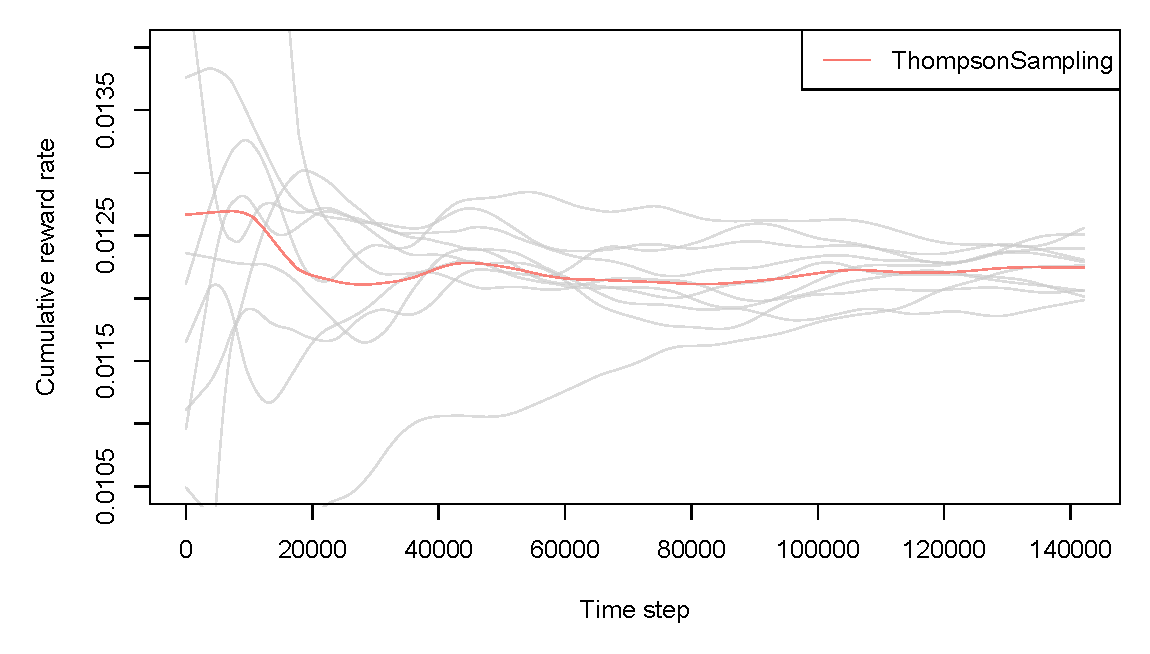
\includegraphics[width=.99\textwidth]{fig/offline_bandit}

      \caption{LinUCBHybridPolicy evaluated with LiSamplingOfflineBandit. The offline bandit samples from 570061 rows with clicks for rewards and the display of one of four “persuasive strategies” to users of an online store representing the offline bandit's four arms. The context is a one dimensional context feature representing whether the page is shown during night or day. }
      \label{fig:offline_bandit}
\end{figure}

\section{Replication of Li et al 2010} \label{repl}

In the current section, we demonstrate how \pkg{contextual} facilitates the comparison of bandit policies on big offline datasets by running a partial replication of \cite{Li2010}'s frequently cited "A Contextual-Bandit Approach to Personalized News Article Recommendation.". The paper describes how the authors made use of offline Yahoo! click-through rate data to evaluate and compare the effectiveness of several context-free and contextual policies---therein introducing both the offline policy evaluator outlined in the previous section and the LinUCB algorithm introduced in section 5.4.

\subsection{Description of the data} \label{datadesc}

The dataset used in the \cite{Li2010} paper has been made available at the Yahoo! lab's website\footnote{At https://webscope.sandbox.yahoo.com/catalog.php?datatype=r\&did=49}. It contains the click-through rate from the Today news module on Yahoo!'s homepage over the course of several days in May 2009, totaling 45,811,883 separate, random and unbiased events.

Each row in the dataset describes an interaction event (click or no click) of users shown a randomly chosen article. Each of these events contains information on (I) six features for each of a varying subset of 19 to 25 articles shown below the the story position drawn from a pool of 217 articles by human editors (II) the id ofthe articles that is randomly chosen to be positioned at the story position at the top of the Today module on Yahoo!'s website (III) six user features, where each event contains another, distinct user (IV) information on whether the user clicked on the article at the story position, or not.

That is, for each event $t$ an article represents one of $k$ arms (that is, one of the 271 articles observed within the course of the 10 days covered by the dataset) with $\mathbb{R}^6$ features $X_{t,a}$ per arm, and another $\mathbb{R}^6$ features $X_{t,u}$ per unique visitor. Together, the flattened outer product of the user and article feature vector creates a $\mathbb{R}^{36}$ feature vector $X_t$ for each user and article pair with the outcome value or reward $r_t$) click (1) or no click (0). For the further details on the data structure and the general setup of the experiment, we refer the reader to \cite{Chu2009} and to the original \cite{Li2010} paper.

\subsection{Data import} \label{dataimp}

As the Yahoo data is too large to fit into memory, we imported most\footnote{The first two CSV files of the Yahoo! dataset are somewhat irregular, as they contain articles with more than six features. We, therefore, decided to leave these two CSV files out of our import, resulting in 37,450,196 imported events, instead of the 45,811,883 events used in the original paper.} of the dataset's CSV files into a MonetDB \citep{IdreosGNMMK12} instance---a fast, open source column-oriented database management system with excellent \proglang{R} support\footnote{MonetDB can be downloaded at https://www.monetdb.org/}. The import script, example import scripts for several other databases (MySQL, SQLite, Postgresql) and all other source code related to this replication can be found in the package's \code{demo/replication_li_2010 directory}.

\subsection{Custom bandit and policies} \label{custom}

With the Yahoo! data imported into our MonetDB server, our next step was the creation of a \code{Bandit} subclass to query the data and the seven \code{Policy} subclasses implementing the policies described in the \cite{Li2010} paper. Though most of these Policies were already implemented in \pkg{contextual}, the fact that only a subset of all 271 articles or arms is shown to a visitor at a time meant we needed to make some minor adaptations to all of the pre-implemented policies to make our policies run smoothly on this continually shifting pool of available arms.

In effect, first, our YahooBandit receives a \code{self$arm_lookup} table with an overview of 271 all arms. The bandit then proceeds to look up the article id's in the lookup table at each time step $t$, and includes the indexes of the currently active arms in the context list:

\begin{Code}
    get_context = function(index) {
      ...
      # Retrieve the index of all arms this row/event.
      arm_indices_this_event   <- seq(10, 184, by = 7)
      article_ids              <- row[arm_indices_this_event]
      article_ids              <- article_ids[!is.na(article_ids)]
      article_ids              <- match(article_ids,self$arm_lookup)
      ...
      contextlist <- list(
        k = self$k,
        d = self$d,
        unique = self$unique, # <-- Indexes of all disjoint arms (user features)
        shared = self$shared, # <-- Indexes of all shared arms (article features)
        arms = article_ids,   # <-- Indexes of arms this event.
        X = X
      )
    }
\end{Code}

These indexes are then picked up by the policy classes, which use the article id's to select and update only the currently active subset of arms. For instance, in YahooEpsilonGreedyPolicy's \code{get_action()}:

\begin{Code}
    get_action = function(t, context) {
      if (runif(1) > self$epsilon) {
        # get the max of context$arms *currently in play*
        max_index            <- context$arms[max_in(theta$mean[context$arms])]
        self$action$choice   <- max_index
      } else {
        # sample from the arms *currently in play*
        self$action$choice   <- sample(context$arms, 1)
      }
      self$action
    }
\end{Code}

Next, we initiated the seven customized policy subclasses (Random, EGreedy, EGreedySeg, LinUCB Dis, LinUCB Hyb, UCB1 and the UCB1Seg\footnote{EGreedy Dis and EGreedy Hyb were too summarily described for us to be able to replicate them with confidence.}) for each of the six (0, 30, 20, 10, 5 and 1 percent) levels of sparsity defined in the original paper. Resulting in $7\times6=42$ Agents, each in their turn added to one Simulation instance which is then run on the offline dataset:

\begin{Code}
simulations             <- 1
horizon                 <- 37.45e6
...
con <- DBI::dbConnect(MonetDB.R(), host=monetdb_host, dbname=monetdb_dbname,
                                   user=monetdb_user, password=monetdb_password)

message(paste0("MonetDB: connection to '",dbListTables(con),"' succesful!"))

arm_lookup_table <-
  as.matrix(DBI::dbGetQuery(con, "SELECT DISTINCT article_id FROM yahoo"))

arm_lookup_table <- rev(as.vector(arm_lookup_table))

bandit <- YahooBandit$new(k = 217L, unique = c(1:6), shared = c(7:12),
                          arm_lookup = arm_lookup_table, host = monetdb_host,
                          dbname = monetdb_dbname, user = monetdb_user,
                          password = monetdb_password, buffer_size = buffer_size)

agents <-
  list (Agent$new(YahooLinUCBDisjointPolicy$new(0.2),
                  bandit, name = "LinUCB Dis",  sparse = 0.99),
        Agent$new(YahooLinUCBHybridPolicy$new(0.2),
                  bandit, name = "LinUCB Hyb",  sparse = 0.99),
        Agent$new(YahooEpsilonGreedyPolicy$new(0.3),
                  bandit, name = "EGreedy",     sparse = 0.99),
        Agent$new(YahooEpsilonGreedySegPolicy$new(0.3),
                  bandit, name = "EGreedySeg",  sparse = 0.99),
        Agent$new(YahooUCB1AlphaPolicy$new(0.4),
                  bandit, name = "UCB1",        sparse = 0.99),
        Agent$new(YahooUCB1AlphaSegPolicy$new(0.4),
                  bandit, name = "UCB1Seg",     sparse = 0.99),
        ...
        Agent$new(YahooRandomPolicy$new(),
                  bandit, name = "Random"))

simulation <- Simulator$new(
    agents,
    simulations = simulations,
    horizon = horizon,
    do_parallel = TRUE,
    worker_max = worker_max,
    reindex = TRUE,
    progress_file = TRUE,
    include_packages = c("MonetDB.R"))

history  <- simulation$run()
...
\end{Code}



\subsection{Results} \label{rslts}

We were able to complete a $7\times6=42$ Agent simulation learning over all of the 37,450,196 events in our database within 22 hours on a 64 core Intel Xeon Unbuntu server with 256GB of memory. We then proceeded to use the results of the first 4.7 million events (following the original paper, representing about a day worth of events) to reproduce \cite{Li2010}'s Figure 4b: "CTRs in evaluation data with varying data sizes in the learning bucket.". Just as the original paper, the replicated Figure \ref{fig:ctr_examples} reports each algorithm’s relative CTR for all of the defined data sparsity levels, that is, each algorithm’s CTR divided by the random policy’s CTR.

\begin{figure}[H]
  \centering
    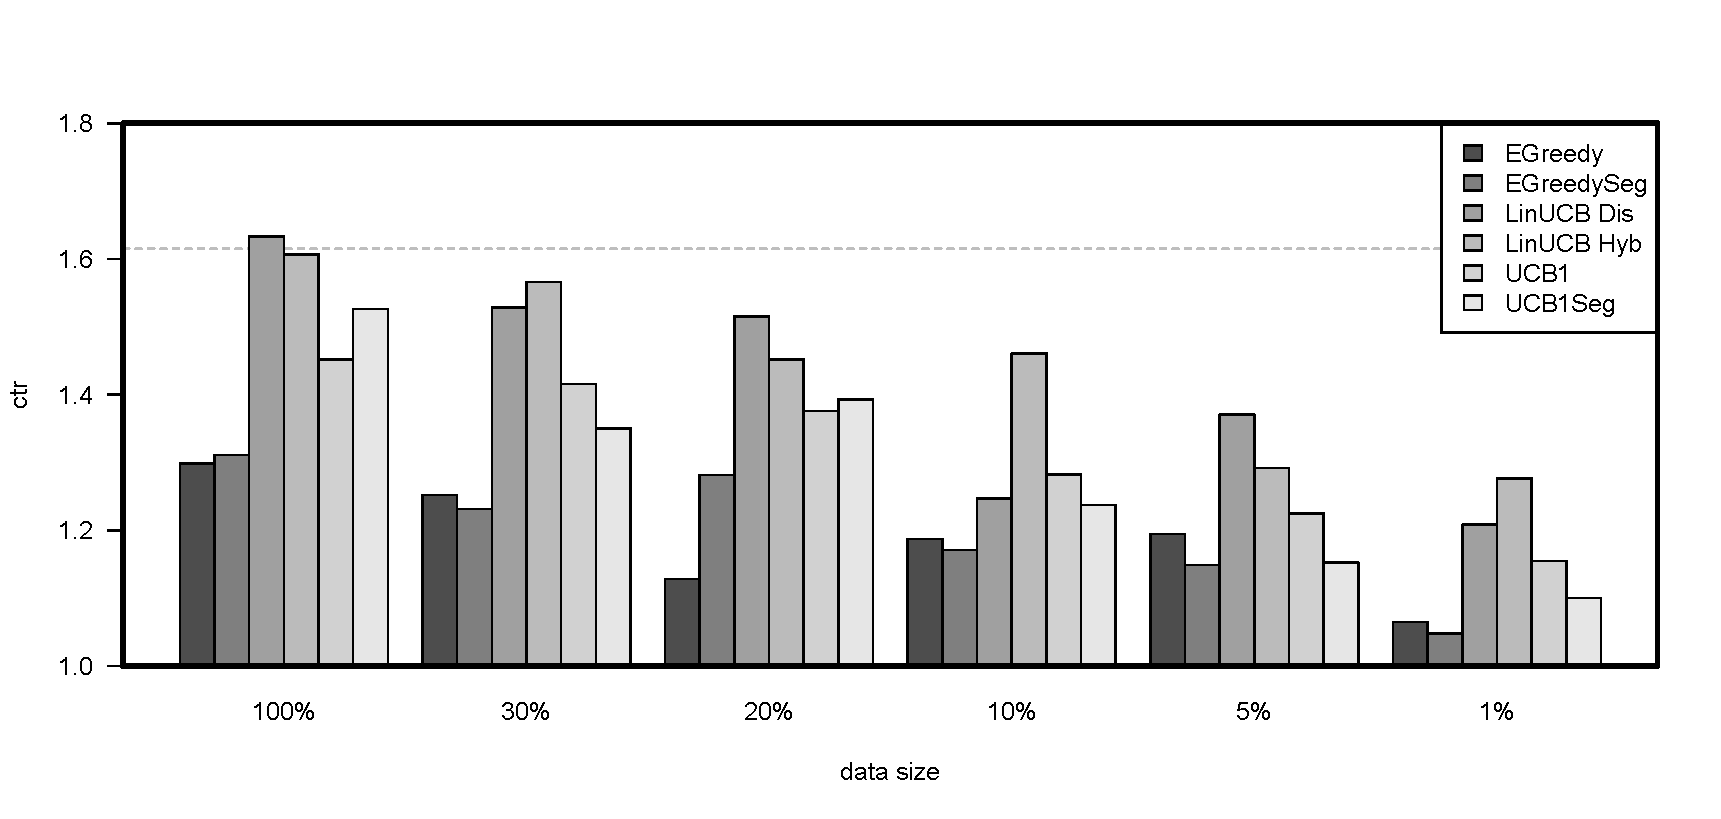
\includegraphics[width=.99\textwidth]{fig/ctr_comparison}
      \caption{Replication of Figure 4b on Yahoo! dataset's day three: "CTRs in evaluation data with varying data sizes in the learning bucket." from \cite{Li2010}.}
      \label{fig:ctr_comparison}
\end{figure}

As can be observed in Figure \ref{fig:ctr_comparison}, after one day of learning, the conclusions of the original paper still stand. First, features again prove to be of use at all levels of sparsity, as LinUCB policies outperform the others consistently. Second, UCB policies generally outperform $\epsilon$-greedy ones. And third, Hybrid LinUCB again shows benefits when the data is small, as can be deduced from it doing better in the 1\% bucket. Still, as we started our simulation on the third day instead of the first, our results are close to, but not quite the same as those reported in the original paper. Particularly the third conclusion, that of the relative advantage of Hybrid LinUCB with sparse data, seems to be less convincing in our Figure \ref{fig:ctr_comparison}.

So we decided to run a simulation that would continue to learn beyond the first day on sparse (1\%) data to test whether Hybrid LinUCB's relative advantage would prove stable over time.

\begin{figure}[H]
  \centering
    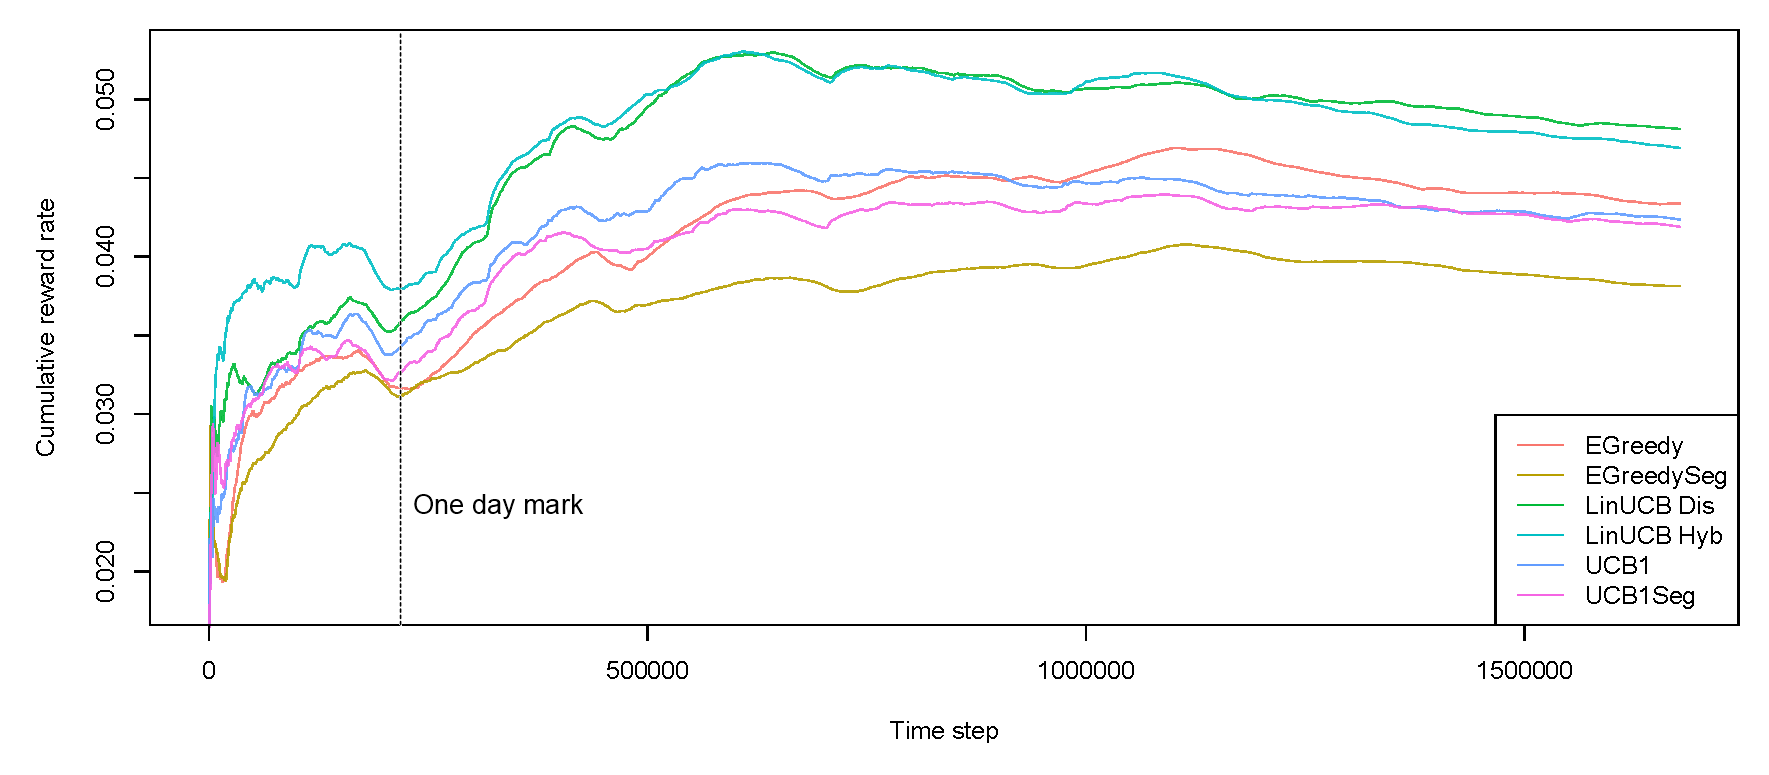
\includegraphics[width=.99\textwidth]{fig/one_day}
      \caption{A plot of the cummulative reward rate (equals click-through rate) for EGreedy, EGreedySeg, LinUCB Dis, LinUCB Hyb, UCB1 and UCB1Seg policies over eight days of events from the Yahoo dataset.}
      \label{fig:one_day}
\end{figure}

From this new Figure \ref{fig:ctr_comparison}, it seems that after one day of training the policies did not settle yet. Looking at the full span of about eight days of learning under 1\% sparse conditions, the advantage of Hybrid LinUCB over Disjoint LinUCB seems to melt away and change into an advantage of the Disjoint version. Also, surprisingly, over the full eight days, the $\epsilon$-greedy policy goes from the worst to third best policy overall, and to best context-free policy---outperforming both context-free UCB policies. Though we intend to further analyze this discrepancy in the near future, for now, these results seem to contradict two out of three conclusions drawn from the original figure---leaving only the first outcome, the superiority of the contextual LinUCB in comparison to several context-free ones, standing. Underlining the benefits of \pkg{contextual}, as it enabled us to replicate and confirm the original \cite{Li2010} paper, and then explore it further with ease. All within about two days of work: extending \code{Bandit} and \code{Policy} classes, simulating all policy classes in parallel on an offline dataset, and plotting and analyzing the results.

\section{Discussion and Future Work} \label{future}

Statistical computational methods, in \proglang{R} or otherwise, are regularly made available through single-use scripts or basic, isolated code packages \citep{Gandrud2016}. Usually, such code examples are meant to give a basic idea of a statistical method, technique or algorithm in the context of a scientific paper \citep{Stodden2013}. Such code examples offer their scientific audience a first inroad towards the comparison and further implementation of their underlying methods \citep{Buckheit1995}. However, when a set of well-researched interrelated algorithms, such as MAB and CMAB policies, find growing academic, practical and commercial adoption, it becomes crucial to offer a more standardized and more accessible way to compare such methods and algorithms \citep{Mesirov2010}.

It is on that premise that we decided to develop the \pkg{contextual} \proglang{R} package---a package that would offer an open bandit framework with easily extensible bandit and policy libraries. To us, it made the most sense to create such a package in \proglang{R} \citep{RCore}, as \proglang{R} is currently the de facto language for the dissemination of new statistical methods, techniques, and algorithms \citep{Tippmann2015}---while it is at the same time finding ever-growing adoption in industry \citep{2012}. The resulting lively exchange of \proglang{R} related code, data, and knowledge between scientists and practitioners offers precisely the kind of cross-pollination that \pkg{contextual} hopes to facilitate.

In making the package publicly available, we hope to further the dissemination and evaluation of both existing and new CMAB policies. By developing the package \proglang{R}, we furthermore hope to offer an arena for the lively exchange of policies between scientists and practitioners---as \proglang{R} has proven itself to be the de facto domain specific computer language in both academia and industry, from the social and medical sciences to statistics and business analytics \citep{Tippmann2015}.

As the package is intended to be usable by practitioners, scientists and students alike, we started our paper with a general introduction to the (contextual) multi-armed bandit problem, followed by a compact formalization. We then demonstrated how our implementation flows naturally from this formalisation, with Agents that cycle Bandits and Policies through four function calls: \code{get_context()}, \code{get_action()}, \code{get_reward()} and \code{set_reward()}. Next, we evaluated some of \pkg{contextual}'s built-in Policies, delved deeper into \pkg{contextual}'s class structure, extended \pkg{contextual}'s \code{Bandit} and \code{Policy} superclasses, demonstrated how to evaluate Policies on offline datasets, and, finally replicated a frequently cited CMAB paper.

Though the package is fully functional and we expect no more changes to its core architecture and API, there is ample room to further improve and extend \pkg{contextual}. We intend to expand \pkg{contextual}'s documentation and tests. We may include more bandit paradigms, such as dueling and combinatorial bandits. We are thinking about replicating some more oft-cited CMAB papers. We expect to add a doubly robust bandit \citep{Dudik2011}. We are interested in growing our policy library---possibly by creating a separate repository where both existing and new CMAB policies are shared, evaluated and compared. Finally, we hope that the package will find an active community of users and developers, organically growing the package in new and unexpected ways and introducing an ever-growing group of people, from business and marketing to the social and medical sciences, to the refined sequential decision strategies offered by contextual bandit policies and algorithms.


%\bibliographystyle{apacite}
\bibliography{jss}

\newpage

\section{Appendix A: UML Diagrams} \label{uml}

\begin{figure}[H]
  \centering
    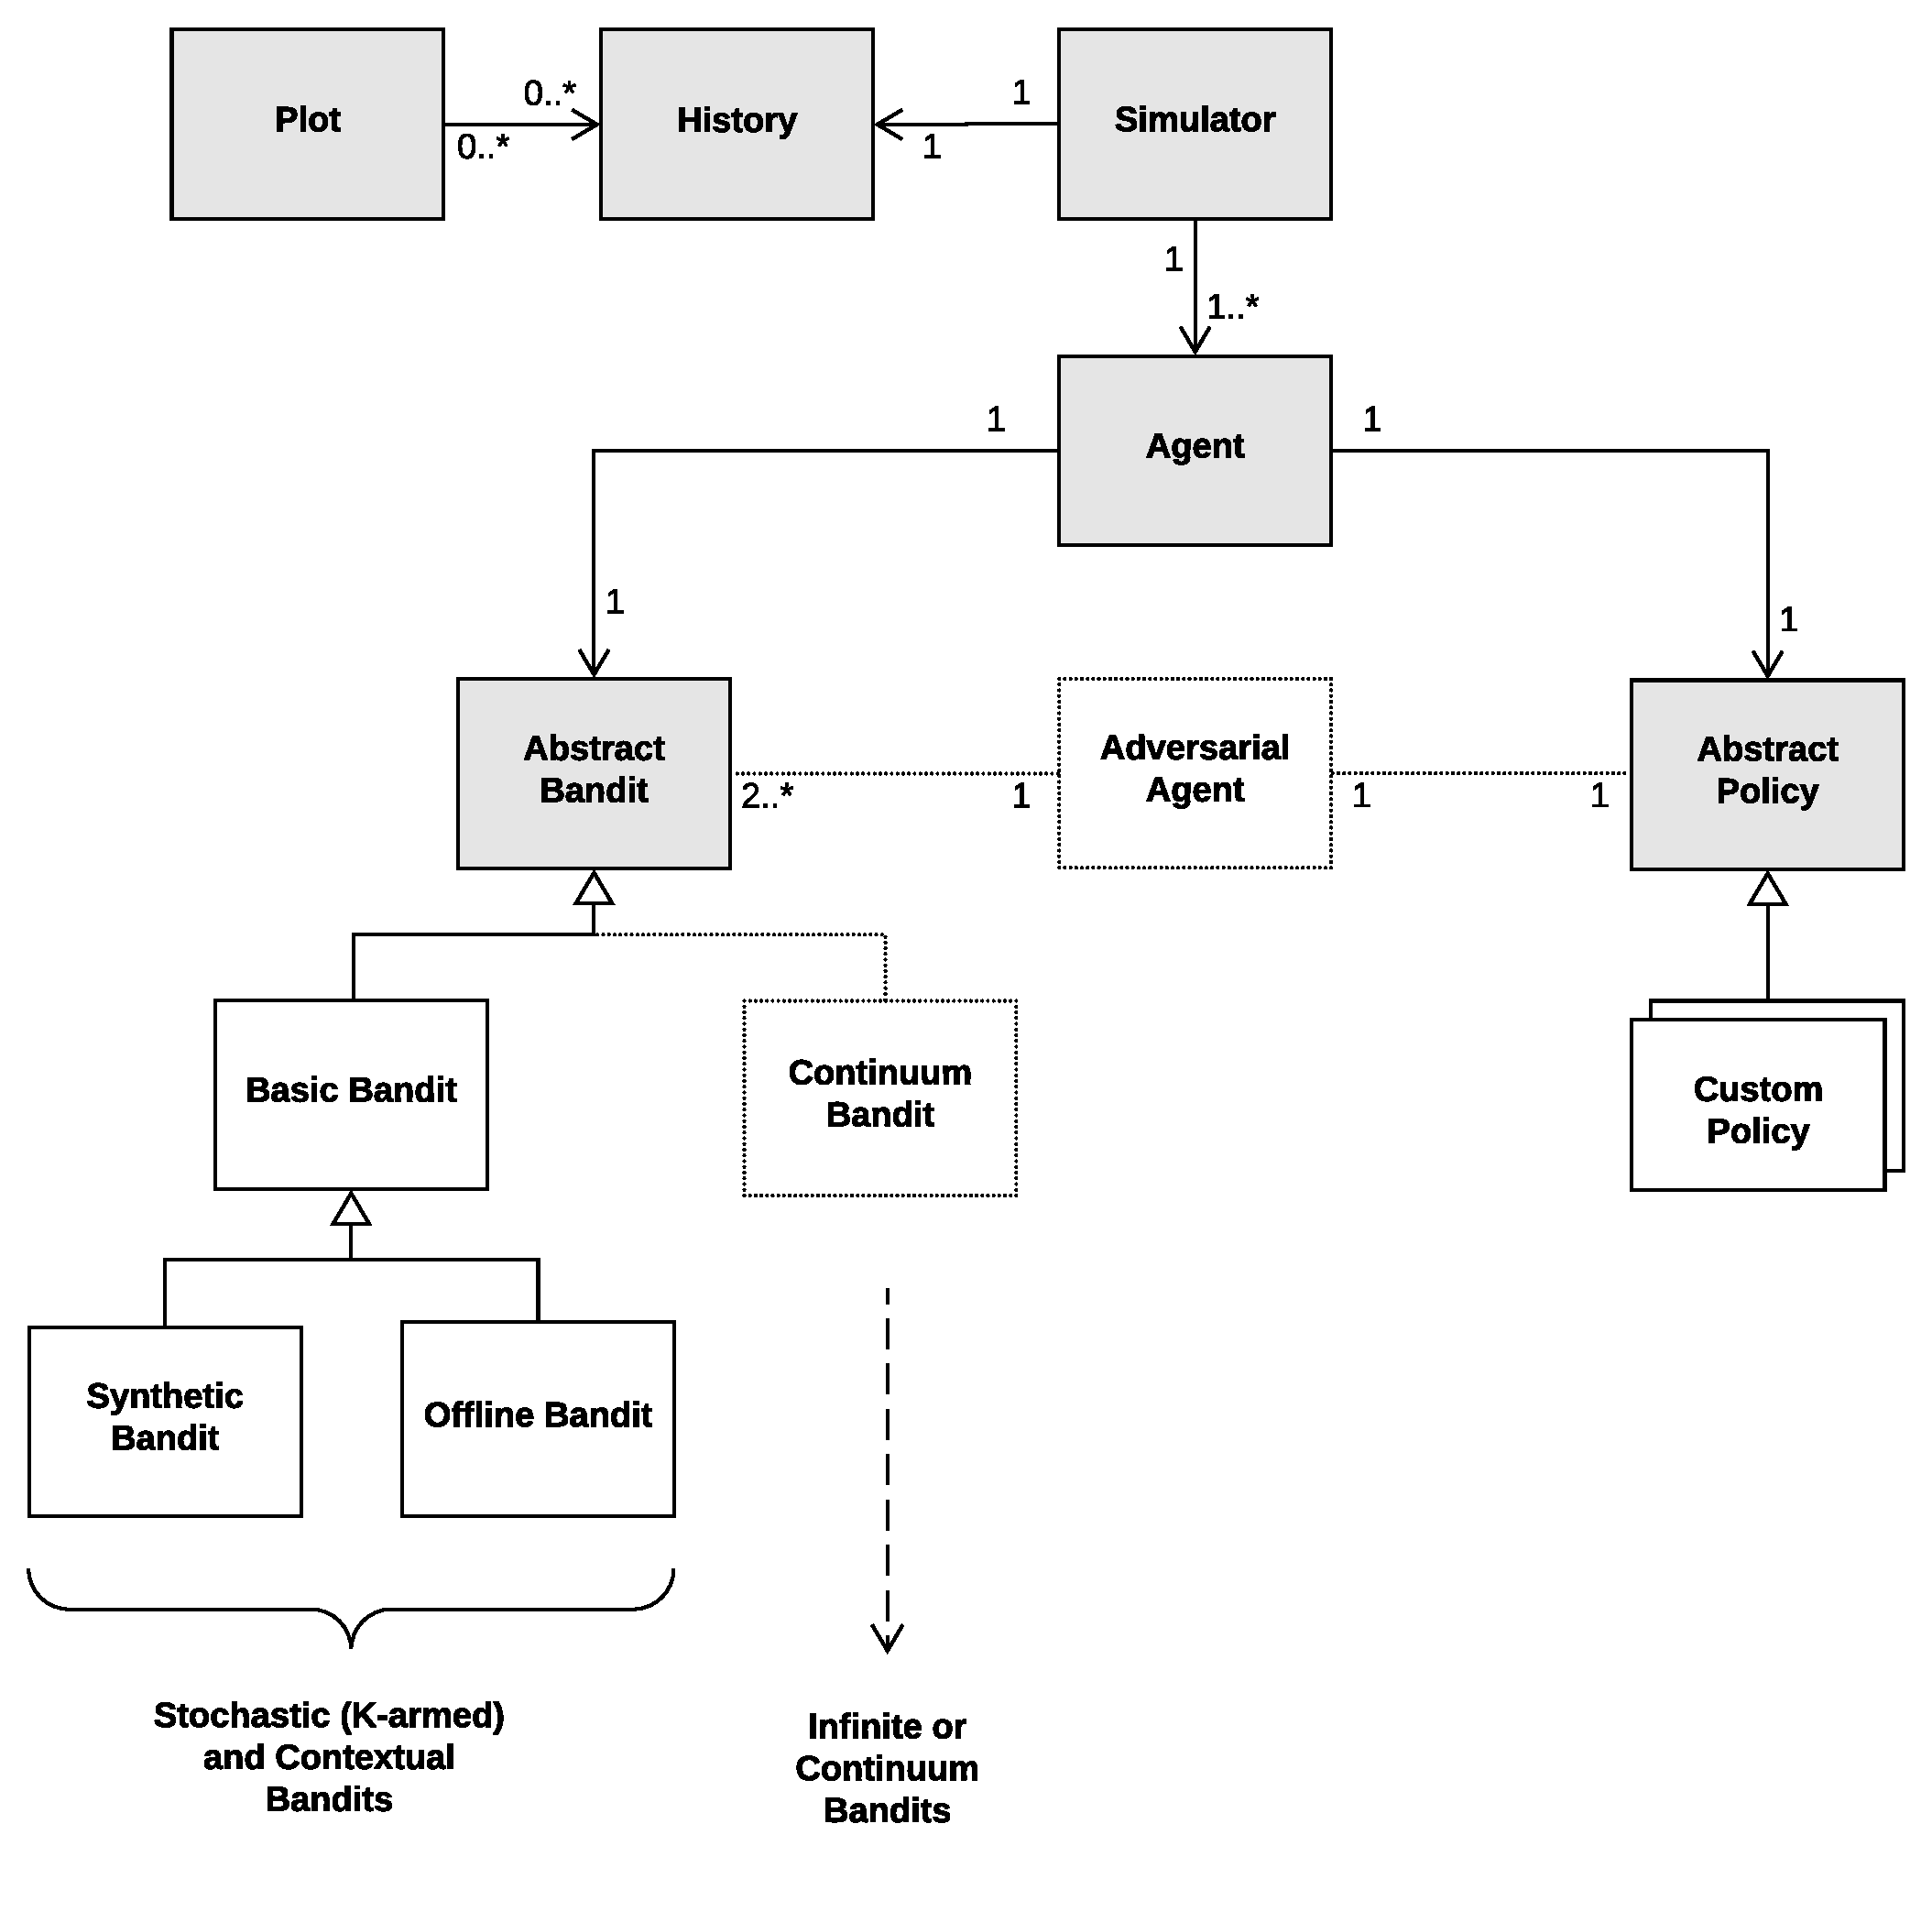
\includegraphics[width=.99\textwidth]{fig/contextual_class}

      \caption{\pkg{contextual} UML Class Diagram}
          \label{fig:contextual_class}
\end{figure}

\begin{figure}[H]
  \centering
    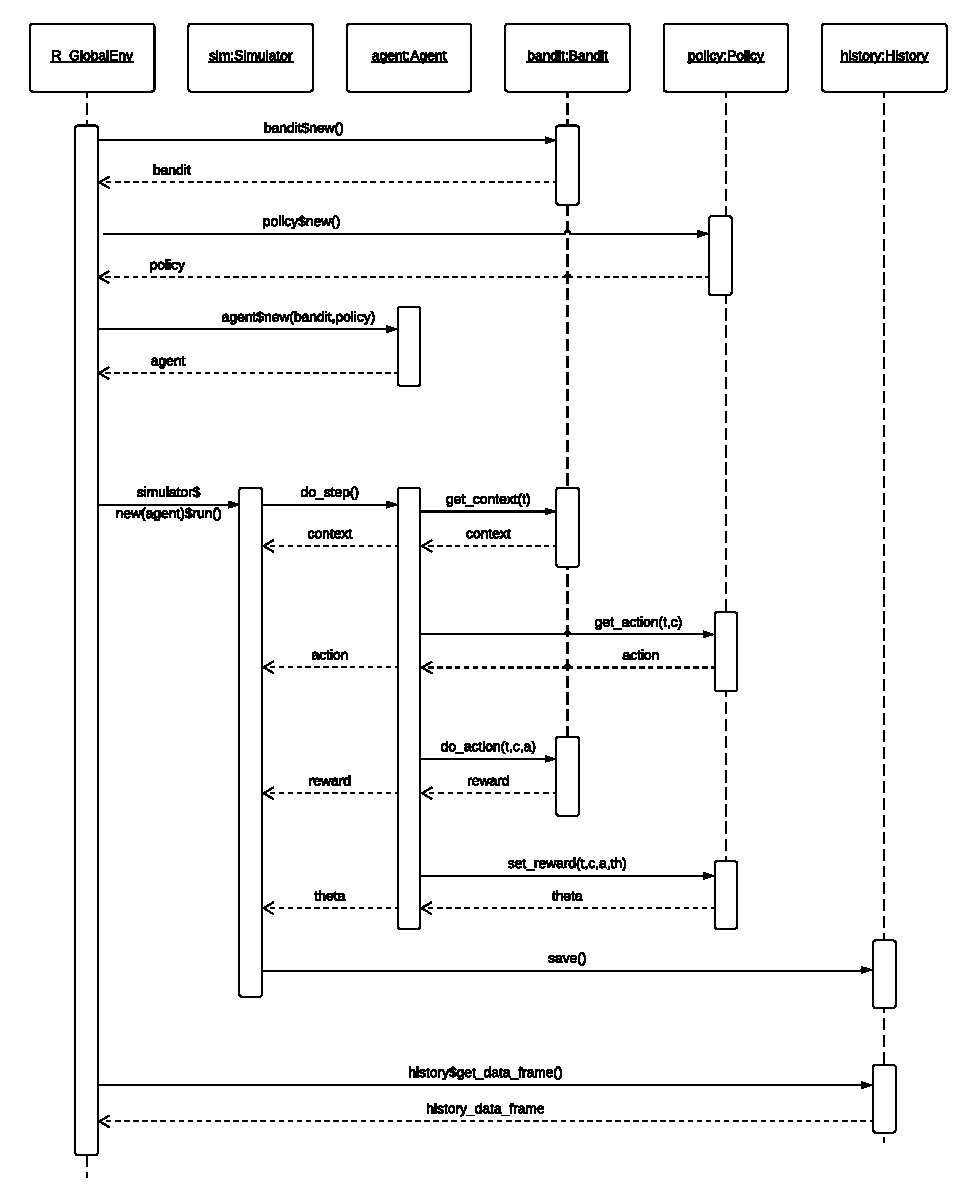
\includegraphics[width=.99\textwidth]{fig/contextual_sequence}

      \caption{\pkg{contextual} UML Sequence Diagram}
      \label{fig:contextual_sequence}
\end{figure}

\end{document}
